\documentclass{article}

\usepackage[final]{neurips_2026}
% The [final] option alone defines no track; set the footer notice to the competition.
\makeatletter
\providecommand{\@trackname}{Technical report, Predictive AI Evaluation Competition (PAIEC), \@neuripsordinal\ Conference on Neural Information Processing Systems (NeurIPS \@neuripsyear).}
\makeatother

\usepackage[utf8]{inputenc}
\usepackage[T1]{fontenc}
\usepackage{hyperref}
\usepackage{url}
\usepackage{booktabs}
\usepackage{amsfonts}
\usepackage{amsmath}
\usepackage{nicefrac}
\usepackage{microtype}
\usepackage{xcolor}
\usepackage{graphicx}
\usepackage{multirow}
\usepackage{array}

% generated by experiments/src/make_macros.py -- do not edit
\newcommand{\NBoot}{1,000}
\newcommand{\SNPairs}{160}
\newcommand{\SConstAlc}{0.2500}
\newcommand{\SConstAlcLo}{0.2500}
\newcommand{\SConstAlcHi}{0.2500}
\newcommand{\SConstEce}{0.111}
\newcommand{\SConstBZero}{0.250}
\newcommand{\SConstBOne}{0.250}
\newcommand{\SConstBThree}{0.250}
\newcommand{\SConstBSeven}{0.250}
\newcommand{\SConstBFifteen}{0.250}
\newcommand{\SConstBThirtyOne}{0.250}
\newcommand{\SEmpAlc}{0.2208}
\newcommand{\SEmpAlcLo}{0.2055}
\newcommand{\SEmpAlcHi}{0.2362}
\newcommand{\SEmpEce}{0.114}
\newcommand{\SEmpBZero}{0.250}
\newcommand{\SEmpBOne}{0.330}
\newcommand{\SEmpBThree}{0.211}
\newcommand{\SEmpBSeven}{0.183}
\newcommand{\SEmpBFifteen}{0.172}
\newcommand{\SEmpBThirtyOne}{0.166}
\newcommand{\SPriorAlc}{0.2148}
\newcommand{\SPriorAlcLo}{0.2040}
\newcommand{\SPriorAlcHi}{0.2251}
\newcommand{\SPriorEce}{0.041}
\newcommand{\SPriorBZero}{0.215}
\newcommand{\SPriorBOne}{0.215}
\newcommand{\SPriorBThree}{0.215}
\newcommand{\SPriorBSeven}{0.215}
\newcommand{\SPriorBFifteen}{0.215}
\newcommand{\SPriorBThirtyOne}{0.215}
\newcommand{\SShrinkAlc}{0.1797}
\newcommand{\SShrinkAlcLo}{0.1691}
\newcommand{\SShrinkAlcHi}{0.1900}
\newcommand{\SShrinkEce}{0.035}
\newcommand{\SShrinkBZero}{0.215}
\newcommand{\SShrinkBOne}{0.201}
\newcommand{\SShrinkBThree}{0.181}
\newcommand{\SShrinkBSeven}{0.169}
\newcommand{\SShrinkBFifteen}{0.162}
\newcommand{\SShrinkBThirtyOne}{0.157}
\newcommand{\SRidgeAlc}{0.1814}
\newcommand{\SRidgeAlcLo}{0.1708}
\newcommand{\SRidgeAlcHi}{0.1918}
\newcommand{\SRidgeEce}{0.029}
\newcommand{\SRidgeBZero}{0.215}
\newcommand{\SRidgeBOne}{0.201}
\newcommand{\SRidgeBThree}{0.181}
\newcommand{\SRidgeBSeven}{0.172}
\newcommand{\SRidgeBFifteen}{0.165}
\newcommand{\SRidgeBThirtyOne}{0.159}
\newcommand{\SKnnAlc}{0.1794}
\newcommand{\SKnnAlcLo}{0.1687}
\newcommand{\SKnnAlcHi}{0.1895}
\newcommand{\SKnnEce}{0.033}
\newcommand{\SKnnBZero}{0.215}
\newcommand{\SKnnBOne}{0.201}
\newcommand{\SKnnBThree}{0.181}
\newcommand{\SKnnBSeven}{0.168}
\newcommand{\SKnnBFifteen}{0.161}
\newcommand{\SKnnBThirtyOne}{0.156}
\newcommand{\SFullAlc}{0.1797}
\newcommand{\SFullAlcLo}{0.1691}
\newcommand{\SFullAlcHi}{0.1900}
\newcommand{\SFullEce}{0.032}
\newcommand{\SFullBZero}{0.215}
\newcommand{\SFullBOne}{0.201}
\newcommand{\SFullBThree}{0.181}
\newcommand{\SFullBSeven}{0.169}
\newcommand{\SFullBFifteen}{0.162}
\newcommand{\SFullBThirtyOne}{0.157}
\newcommand{\SOrRateAlc}{0.1598}
\newcommand{\SOrRateAlcLo}{0.1483}
\newcommand{\SOrRateAlcHi}{0.1710}
\newcommand{\SOrRateEce}{0.000}
\newcommand{\SOrRateBZero}{0.160}
\newcommand{\SOrRateBOne}{0.160}
\newcommand{\SOrRateBThree}{0.160}
\newcommand{\SOrRateBSeven}{0.160}
\newcommand{\SOrRateBFifteen}{0.160}
\newcommand{\SOrRateBThirtyOne}{0.160}
\newcommand{\SOrPAlc}{0.1379}
\newcommand{\SOrPAlcLo}{0.1280}
\newcommand{\SOrPAlcHi}{0.1482}
\newcommand{\SOrPEce}{0.007}
\newcommand{\SOrPBZero}{0.138}
\newcommand{\SOrPBOne}{0.138}
\newcommand{\SOrPBThree}{0.138}
\newcommand{\SOrPBSeven}{0.138}
\newcommand{\SOrPBFifteen}{0.138}
\newcommand{\SOrPBThirtyOne}{0.138}
\newcommand{\SPairFullConstMean}{-0.0703}
\newcommand{\SPairFullConstLo}{-0.0805}
\newcommand{\SPairFullConstHi}{-0.0592}
\newcommand{\SPairFullConstSig}{significant}
\newcommand{\SPairFullConstFrac}{84\%}
\newcommand{\SPairFullEmpMean}{-0.0411}
\newcommand{\SPairFullEmpLo}{-0.0488}
\newcommand{\SPairFullEmpHi}{-0.0339}
\newcommand{\SPairFullEmpSig}{significant}
\newcommand{\SPairFullEmpFrac}{82\%}
\newcommand{\SPairFullShrinkMean}{+0.0000}
\newcommand{\SPairFullShrinkLo}{-0.0002}
\newcommand{\SPairFullShrinkHi}{+0.0003}
\newcommand{\SPairFullShrinkSig}{not significant}
\newcommand{\SPairFullShrinkFrac}{26\%}
\newcommand{\SPairFullKnnMean}{+0.0004}
\newcommand{\SPairFullKnnLo}{+0.0002}
\newcommand{\SPairFullKnnHi}{+0.0006}
\newcommand{\SPairFullKnnSig}{significant}
\newcommand{\SPairFullKnnFrac}{31\%}
\newcommand{\SPairFullRidgeMean}{-0.0017}
\newcommand{\SPairFullRidgeLo}{-0.0023}
\newcommand{\SPairFullRidgeHi}{-0.0010}
\newcommand{\SPairFullRidgeSig}{significant}
\newcommand{\SPairFullRidgeFrac}{72\%}
\newcommand{\SPairShrinkConstMean}{-0.0703}
\newcommand{\SPairShrinkConstLo}{-0.0805}
\newcommand{\SPairShrinkConstHi}{-0.0592}
\newcommand{\SPairShrinkConstSig}{significant}
\newcommand{\SPairShrinkConstFrac}{86\%}
\newcommand{\SPairShrinkEmpMean}{-0.0411}
\newcommand{\SPairShrinkEmpLo}{-0.0490}
\newcommand{\SPairShrinkEmpHi}{-0.0339}
\newcommand{\SPairShrinkEmpSig}{significant}
\newcommand{\SPairShrinkEmpFrac}{82\%}
\newcommand{\SPairKnnShrinkMean}{-0.0003}
\newcommand{\SPairKnnShrinkLo}{-0.0005}
\newcommand{\SPairKnnShrinkHi}{-0.0001}
\newcommand{\SPairKnnShrinkSig}{significant}
\newcommand{\SPairKnnShrinkFrac}{66\%}
\newcommand{\SPairRidgeShrinkMean}{+0.0017}
\newcommand{\SPairRidgeShrinkLo}{+0.0011}
\newcommand{\SPairRidgeShrinkHi}{+0.0024}
\newcommand{\SPairRidgeShrinkSig}{significant}
\newcommand{\SPairRidgeShrinkFrac}{32\%}
\newcommand{\SPairPriorConstMean}{-0.0352}
\newcommand{\SPairPriorConstLo}{-0.0454}
\newcommand{\SPairPriorConstHi}{-0.0244}
\newcommand{\SPairPriorConstSig}{significant}
\newcommand{\SPairPriorConstFrac}{69\%}
\newcommand{\SPairShrinkPriorMean}{-0.0351}
\newcommand{\SPairShrinkPriorLo}{-0.0415}
\newcommand{\SPairShrinkPriorHi}{-0.0285}
\newcommand{\SPairShrinkPriorSig}{significant}
\newcommand{\SPairShrinkPriorFrac}{76\%}
\newcommand{\SPairEmpConstMean}{-0.0292}
\newcommand{\SPairEmpConstLo}{-0.0442}
\newcommand{\SPairEmpConstHi}{-0.0129}
\newcommand{\SPairEmpConstSig}{significant}
\newcommand{\SPairEmpConstFrac}{51\%}
\newcommand{\SPairFullShrinkBZeroMean}{+0.000}
\newcommand{\SPairFullShrinkBZeroLo}{+0.000}
\newcommand{\SPairFullShrinkBZeroHi}{+0.000}
\newcommand{\SPairFullShrinkBZeroSig}{not significant}
\newcommand{\SPairFullShrinkBZeroFrac}{0\%}
\newcommand{\SPairFullShrinkBOneMean}{+0.000}
\newcommand{\SPairFullShrinkBOneLo}{+0.000}
\newcommand{\SPairFullShrinkBOneHi}{+0.000}
\newcommand{\SPairFullShrinkBOneSig}{not significant}
\newcommand{\SPairFullShrinkBOneFrac}{0\%}
\newcommand{\SPairFullShrinkBThreeMean}{+0.000}
\newcommand{\SPairFullShrinkBThreeLo}{+0.000}
\newcommand{\SPairFullShrinkBThreeHi}{+0.000}
\newcommand{\SPairFullShrinkBThreeSig}{not significant}
\newcommand{\SPairFullShrinkBThreeFrac}{0\%}
\newcommand{\SPairFullShrinkBSevenMean}{+0.000}
\newcommand{\SPairFullShrinkBSevenLo}{-0.001}
\newcommand{\SPairFullShrinkBSevenHi}{+0.001}
\newcommand{\SPairFullShrinkBSevenSig}{not significant}
\newcommand{\SPairFullShrinkBSevenFrac}{21\%}
\newcommand{\SPairFullShrinkBFifteenMean}{+0.000}
\newcommand{\SPairFullShrinkBFifteenLo}{-0.000}
\newcommand{\SPairFullShrinkBFifteenHi}{+0.001}
\newcommand{\SPairFullShrinkBFifteenSig}{not significant}
\newcommand{\SPairFullShrinkBFifteenFrac}{12\%}
\newcommand{\SPairFullShrinkBThirtyOneMean}{-0.000}
\newcommand{\SPairFullShrinkBThirtyOneLo}{-0.001}
\newcommand{\SPairFullShrinkBThirtyOneHi}{+0.000}
\newcommand{\SPairFullShrinkBThirtyOneSig}{not significant}
\newcommand{\SPairFullShrinkBThirtyOneFrac}{8\%}
\newcommand{\SPairShrinkConstBZeroMean}{-0.035}
\newcommand{\SPairShrinkConstBZeroLo}{-0.046}
\newcommand{\SPairShrinkConstBZeroHi}{-0.025}
\newcommand{\SPairShrinkConstBZeroSig}{significant}
\newcommand{\SPairShrinkConstBZeroFrac}{69\%}
\newcommand{\SPairShrinkConstBOneMean}{-0.049}
\newcommand{\SPairShrinkConstBOneLo}{-0.062}
\newcommand{\SPairShrinkConstBOneHi}{-0.036}
\newcommand{\SPairShrinkConstBOneSig}{significant}
\newcommand{\SPairShrinkConstBOneFrac}{79\%}
\newcommand{\SPairShrinkConstBThreeMean}{-0.069}
\newcommand{\SPairShrinkConstBThreeLo}{-0.081}
\newcommand{\SPairShrinkConstBThreeHi}{-0.056}
\newcommand{\SPairShrinkConstBThreeSig}{significant}
\newcommand{\SPairShrinkConstBThreeFrac}{83\%}
\newcommand{\SPairShrinkConstBSevenMean}{-0.081}
\newcommand{\SPairShrinkConstBSevenLo}{-0.093}
\newcommand{\SPairShrinkConstBSevenHi}{-0.070}
\newcommand{\SPairShrinkConstBSevenSig}{significant}
\newcommand{\SPairShrinkConstBSevenFrac}{92\%}
\newcommand{\SPairShrinkConstBFifteenMean}{-0.088}
\newcommand{\SPairShrinkConstBFifteenLo}{-0.100}
\newcommand{\SPairShrinkConstBFifteenHi}{-0.076}
\newcommand{\SPairShrinkConstBFifteenSig}{significant}
\newcommand{\SPairShrinkConstBFifteenFrac}{88\%}
\newcommand{\SPairShrinkConstBThirtyOneMean}{-0.093}
\newcommand{\SPairShrinkConstBThirtyOneLo}{-0.105}
\newcommand{\SPairShrinkConstBThirtyOneHi}{-0.082}
\newcommand{\SPairShrinkConstBThirtyOneSig}{significant}
\newcommand{\SPairShrinkConstBThirtyOneFrac}{93\%}
\newcommand{\SPairFullConstBZeroMean}{-0.035}
\newcommand{\SPairFullConstBZeroLo}{-0.046}
\newcommand{\SPairFullConstBZeroHi}{-0.025}
\newcommand{\SPairFullConstBZeroSig}{significant}
\newcommand{\SPairFullConstBZeroFrac}{69\%}
\newcommand{\SPairFullConstBOneMean}{-0.049}
\newcommand{\SPairFullConstBOneLo}{-0.062}
\newcommand{\SPairFullConstBOneHi}{-0.036}
\newcommand{\SPairFullConstBOneSig}{significant}
\newcommand{\SPairFullConstBOneFrac}{79\%}
\newcommand{\SPairFullConstBThreeMean}{-0.069}
\newcommand{\SPairFullConstBThreeLo}{-0.081}
\newcommand{\SPairFullConstBThreeHi}{-0.056}
\newcommand{\SPairFullConstBThreeSig}{significant}
\newcommand{\SPairFullConstBThreeFrac}{83\%}
\newcommand{\SPairFullConstBSevenMean}{-0.081}
\newcommand{\SPairFullConstBSevenLo}{-0.093}
\newcommand{\SPairFullConstBSevenHi}{-0.070}
\newcommand{\SPairFullConstBSevenSig}{significant}
\newcommand{\SPairFullConstBSevenFrac}{91\%}
\newcommand{\SPairFullConstBFifteenMean}{-0.088}
\newcommand{\SPairFullConstBFifteenLo}{-0.100}
\newcommand{\SPairFullConstBFifteenHi}{-0.076}
\newcommand{\SPairFullConstBFifteenSig}{significant}
\newcommand{\SPairFullConstBFifteenFrac}{88\%}
\newcommand{\SPairFullConstBThirtyOneMean}{-0.093}
\newcommand{\SPairFullConstBThirtyOneLo}{-0.105}
\newcommand{\SPairFullConstBThirtyOneHi}{-0.082}
\newcommand{\SPairFullConstBThirtyOneSig}{significant}
\newcommand{\SPairFullConstBThirtyOneFrac}{94\%}
\newcommand{\SHeadroomRate}{0.0199}
\newcommand{\SHeadroomItem}{0.0219}
\newcommand{\SHeadroomRateBZero}{0.055}
\newcommand{\SHeadroomRateBOne}{0.041}
\newcommand{\SHeadroomRateBThree}{0.022}
\newcommand{\SHeadroomRateBSeven}{0.009}
\newcommand{\SHeadroomRateBFifteen}{0.002}
\newcommand{\SHeadroomRateBThirtyOne}{-0.003}
\newcommand{\SFullVsOrRate}{0.0200}
\newcommand{\RNPairs}{15}
\newcommand{\RConstAlc}{0.2500}
\newcommand{\RConstAlcLo}{0.2500}
\newcommand{\RConstAlcHi}{0.2500}
\newcommand{\RConstEce}{0.135}
\newcommand{\RConstBZero}{0.250}
\newcommand{\RConstBOne}{0.250}
\newcommand{\RConstBThree}{0.250}
\newcommand{\RConstBSeven}{0.250}
\newcommand{\RConstBFifteen}{0.250}
\newcommand{\RConstBThirtyOne}{0.250}
\newcommand{\REmpAlc}{0.2745}
\newcommand{\REmpAlcLo}{0.2302}
\newcommand{\REmpAlcHi}{0.3117}
\newcommand{\REmpEce}{0.152}
\newcommand{\REmpBZero}{0.250}
\newcommand{\REmpBOne}{0.468}
\newcommand{\REmpBThree}{0.241}
\newcommand{\REmpBSeven}{0.228}
\newcommand{\REmpBFifteen}{0.209}
\newcommand{\REmpBThirtyOne}{0.202}
\newcommand{\RPriorAlc}{0.2330}
\newcommand{\RPriorAlcLo}{0.2184}
\newcommand{\RPriorAlcHi}{0.2491}
\newcommand{\RPriorEce}{0.071}
\newcommand{\RPriorBZero}{0.233}
\newcommand{\RPriorBOne}{0.233}
\newcommand{\RPriorBThree}{0.233}
\newcommand{\RPriorBSeven}{0.233}
\newcommand{\RPriorBFifteen}{0.233}
\newcommand{\RPriorBThirtyOne}{0.233}
\newcommand{\RShrinkAlc}{0.2187}
\newcommand{\RShrinkAlcLo}{0.1925}
\newcommand{\RShrinkAlcHi}{0.2416}
\newcommand{\RShrinkEce}{0.048}
\newcommand{\RShrinkBZero}{0.233}
\newcommand{\RShrinkBOne}{0.241}
\newcommand{\RShrinkBThree}{0.217}
\newcommand{\RShrinkBSeven}{0.212}
\newcommand{\RShrinkBFifteen}{0.206}
\newcommand{\RShrinkBThirtyOne}{0.201}
\newcommand{\RRidgeAlc}{0.2162}
\newcommand{\RRidgeAlcLo}{0.1919}
\newcommand{\RRidgeAlcHi}{0.2367}
\newcommand{\RRidgeEce}{0.046}
\newcommand{\RRidgeBZero}{0.233}
\newcommand{\RRidgeBOne}{0.241}
\newcommand{\RRidgeBThree}{0.217}
\newcommand{\RRidgeBSeven}{0.212}
\newcommand{\RRidgeBFifteen}{0.199}
\newcommand{\RRidgeBThirtyOne}{0.188}
\newcommand{\RKnnAlc}{0.2189}
\newcommand{\RKnnAlcLo}{0.1924}
\newcommand{\RKnnAlcHi}{0.2420}
\newcommand{\RKnnEce}{0.046}
\newcommand{\RKnnBZero}{0.233}
\newcommand{\RKnnBOne}{0.241}
\newcommand{\RKnnBThree}{0.217}
\newcommand{\RKnnBSeven}{0.212}
\newcommand{\RKnnBFifteen}{0.207}
\newcommand{\RKnnBThirtyOne}{0.201}
\newcommand{\RFullAlc}{0.2183}
\newcommand{\RFullAlcLo}{0.1923}
\newcommand{\RFullAlcHi}{0.2410}
\newcommand{\RFullEce}{0.046}
\newcommand{\RFullBZero}{0.233}
\newcommand{\RFullBOne}{0.241}
\newcommand{\RFullBThree}{0.217}
\newcommand{\RFullBSeven}{0.211}
\newcommand{\RFullBFifteen}{0.206}
\newcommand{\RFullBThirtyOne}{0.199}
\newcommand{\ROrRateAlc}{0.1966}
\newcommand{\ROrRateAlcLo}{0.1685}
\newcommand{\ROrRateAlcHi}{0.2215}
\newcommand{\ROrRateEce}{0.000}
\newcommand{\ROrRateBZero}{0.197}
\newcommand{\ROrRateBOne}{0.197}
\newcommand{\ROrRateBThree}{0.197}
\newcommand{\ROrRateBSeven}{0.197}
\newcommand{\ROrRateBFifteen}{0.197}
\newcommand{\ROrRateBThirtyOne}{0.197}
\newcommand{\ROrPAlc}{\textbf{??}}
\newcommand{\ROrPAlcLo}{\textbf{??}}
\newcommand{\ROrPAlcHi}{\textbf{??}}
\newcommand{\ROrPEce}{\textbf{??}}
\newcommand{\ROrPBZero}{\textbf{??}}
\newcommand{\ROrPBOne}{\textbf{??}}
\newcommand{\ROrPBThree}{\textbf{??}}
\newcommand{\ROrPBSeven}{\textbf{??}}
\newcommand{\ROrPBFifteen}{\textbf{??}}
\newcommand{\ROrPBThirtyOne}{\textbf{??}}
\newcommand{\RPairFullConstMean}{-0.0317}
\newcommand{\RPairFullConstLo}{-0.0574}
\newcommand{\RPairFullConstHi}{-0.0104}
\newcommand{\RPairFullConstSig}{significant}
\newcommand{\RPairFullConstFrac}{73\%}
\newcommand{\RPairFullEmpMean}{-0.0562}
\newcommand{\RPairFullEmpLo}{-0.0771}
\newcommand{\RPairFullEmpHi}{-0.0351}
\newcommand{\RPairFullEmpSig}{significant}
\newcommand{\RPairFullEmpFrac}{80\%}
\newcommand{\RPairFullShrinkMean}{-0.0004}
\newcommand{\RPairFullShrinkLo}{-0.0013}
\newcommand{\RPairFullShrinkHi}{+0.0004}
\newcommand{\RPairFullShrinkSig}{not significant}
\newcommand{\RPairFullShrinkFrac}{27\%}
\newcommand{\RPairFullKnnMean}{-0.0006}
\newcommand{\RPairFullKnnLo}{-0.0015}
\newcommand{\RPairFullKnnHi}{+0.0004}
\newcommand{\RPairFullKnnSig}{not significant}
\newcommand{\RPairFullKnnFrac}{67\%}
\newcommand{\RPairFullRidgeMean}{+0.0021}
\newcommand{\RPairFullRidgeLo}{-0.0014}
\newcommand{\RPairFullRidgeHi}{+0.0053}
\newcommand{\RPairFullRidgeSig}{not significant}
\newcommand{\RPairFullRidgeFrac}{33\%}
\newcommand{\RPairShrinkConstMean}{-0.0313}
\newcommand{\RPairShrinkConstLo}{-0.0573}
\newcommand{\RPairShrinkConstHi}{-0.0102}
\newcommand{\RPairShrinkConstSig}{significant}
\newcommand{\RPairShrinkConstFrac}{73\%}
\newcommand{\RPairShrinkEmpMean}{-0.0558}
\newcommand{\RPairShrinkEmpLo}{-0.0766}
\newcommand{\RPairShrinkEmpHi}{-0.0349}
\newcommand{\RPairShrinkEmpSig}{significant}
\newcommand{\RPairShrinkEmpFrac}{80\%}
\newcommand{\RPairKnnShrinkMean}{+0.0002}
\newcommand{\RPairKnnShrinkLo}{-0.0007}
\newcommand{\RPairKnnShrinkHi}{+0.0011}
\newcommand{\RPairKnnShrinkSig}{not significant}
\newcommand{\RPairKnnShrinkFrac}{40\%}
\newcommand{\RPairRidgeShrinkMean}{-0.0025}
\newcommand{\RPairRidgeShrinkLo}{-0.0062}
\newcommand{\RPairRidgeShrinkHi}{+0.0015}
\newcommand{\RPairRidgeShrinkSig}{not significant}
\newcommand{\RPairRidgeShrinkFrac}{67\%}
\newcommand{\RPairPriorConstMean}{-0.0170}
\newcommand{\RPairPriorConstLo}{-0.0315}
\newcommand{\RPairPriorConstHi}{-0.0032}
\newcommand{\RPairPriorConstSig}{significant}
\newcommand{\RPairPriorConstFrac}{80\%}
\newcommand{\RPairShrinkPriorMean}{-0.0143}
\newcommand{\RPairShrinkPriorLo}{-0.0307}
\newcommand{\RPairShrinkPriorHi}{+0.0002}
\newcommand{\RPairShrinkPriorSig}{not significant}
\newcommand{\RPairShrinkPriorFrac}{53\%}
\newcommand{\RPairEmpConstMean}{+0.0245}
\newcommand{\RPairEmpConstLo}{-0.0200}
\newcommand{\RPairEmpConstHi}{+0.0608}
\newcommand{\RPairEmpConstSig}{not significant}
\newcommand{\RPairEmpConstFrac}{20\%}
\newcommand{\RPairFullShrinkBZeroMean}{+0.000}
\newcommand{\RPairFullShrinkBZeroLo}{+0.000}
\newcommand{\RPairFullShrinkBZeroHi}{+0.000}
\newcommand{\RPairFullShrinkBZeroSig}{not significant}
\newcommand{\RPairFullShrinkBZeroFrac}{0\%}
\newcommand{\RPairFullShrinkBOneMean}{+0.000}
\newcommand{\RPairFullShrinkBOneLo}{+0.000}
\newcommand{\RPairFullShrinkBOneHi}{+0.000}
\newcommand{\RPairFullShrinkBOneSig}{not significant}
\newcommand{\RPairFullShrinkBOneFrac}{0\%}
\newcommand{\RPairFullShrinkBThreeMean}{+0.000}
\newcommand{\RPairFullShrinkBThreeLo}{+0.000}
\newcommand{\RPairFullShrinkBThreeHi}{+0.000}
\newcommand{\RPairFullShrinkBThreeSig}{not significant}
\newcommand{\RPairFullShrinkBThreeFrac}{0\%}
\newcommand{\RPairFullShrinkBSevenMean}{-0.001}
\newcommand{\RPairFullShrinkBSevenLo}{-0.004}
\newcommand{\RPairFullShrinkBSevenHi}{+0.001}
\newcommand{\RPairFullShrinkBSevenSig}{not significant}
\newcommand{\RPairFullShrinkBSevenFrac}{13\%}
\newcommand{\RPairFullShrinkBFifteenMean}{-0.000}
\newcommand{\RPairFullShrinkBFifteenLo}{-0.000}
\newcommand{\RPairFullShrinkBFifteenHi}{+0.000}
\newcommand{\RPairFullShrinkBFifteenSig}{not significant}
\newcommand{\RPairFullShrinkBFifteenFrac}{7\%}
\newcommand{\RPairFullShrinkBThirtyOneMean}{-0.002}
\newcommand{\RPairFullShrinkBThirtyOneLo}{-0.010}
\newcommand{\RPairFullShrinkBThirtyOneHi}{+0.004}
\newcommand{\RPairFullShrinkBThirtyOneSig}{not significant}
\newcommand{\RPairFullShrinkBThirtyOneFrac}{7\%}
\newcommand{\RPairShrinkConstBZeroMean}{-0.017}
\newcommand{\RPairShrinkConstBZeroLo}{-0.032}
\newcommand{\RPairShrinkConstBZeroHi}{-0.003}
\newcommand{\RPairShrinkConstBZeroSig}{significant}
\newcommand{\RPairShrinkConstBZeroFrac}{80\%}
\newcommand{\RPairShrinkConstBOneMean}{-0.009}
\newcommand{\RPairShrinkConstBOneLo}{-0.039}
\newcommand{\RPairShrinkConstBOneHi}{+0.018}
\newcommand{\RPairShrinkConstBOneSig}{not significant}
\newcommand{\RPairShrinkConstBOneFrac}{47\%}
\newcommand{\RPairShrinkConstBThreeMean}{-0.033}
\newcommand{\RPairShrinkConstBThreeLo}{-0.061}
\newcommand{\RPairShrinkConstBThreeHi}{-0.010}
\newcommand{\RPairShrinkConstBThreeSig}{significant}
\newcommand{\RPairShrinkConstBThreeFrac}{80\%}
\newcommand{\RPairShrinkConstBSevenMean}{-0.038}
\newcommand{\RPairShrinkConstBSevenLo}{-0.070}
\newcommand{\RPairShrinkConstBSevenHi}{-0.011}
\newcommand{\RPairShrinkConstBSevenSig}{significant}
\newcommand{\RPairShrinkConstBSevenFrac}{67\%}
\newcommand{\RPairShrinkConstBFifteenMean}{-0.044}
\newcommand{\RPairShrinkConstBFifteenLo}{-0.073}
\newcommand{\RPairShrinkConstBFifteenHi}{-0.018}
\newcommand{\RPairShrinkConstBFifteenSig}{significant}
\newcommand{\RPairShrinkConstBFifteenFrac}{67\%}
\newcommand{\RPairShrinkConstBThirtyOneMean}{-0.049}
\newcommand{\RPairShrinkConstBThirtyOneLo}{-0.079}
\newcommand{\RPairShrinkConstBThirtyOneHi}{-0.025}
\newcommand{\RPairShrinkConstBThirtyOneSig}{significant}
\newcommand{\RPairShrinkConstBThirtyOneFrac}{80\%}
\newcommand{\RPairFullConstBZeroMean}{-0.017}
\newcommand{\RPairFullConstBZeroLo}{-0.032}
\newcommand{\RPairFullConstBZeroHi}{-0.003}
\newcommand{\RPairFullConstBZeroSig}{significant}
\newcommand{\RPairFullConstBZeroFrac}{80\%}
\newcommand{\RPairFullConstBOneMean}{-0.009}
\newcommand{\RPairFullConstBOneLo}{-0.039}
\newcommand{\RPairFullConstBOneHi}{+0.018}
\newcommand{\RPairFullConstBOneSig}{not significant}
\newcommand{\RPairFullConstBOneFrac}{47\%}
\newcommand{\RPairFullConstBThreeMean}{-0.033}
\newcommand{\RPairFullConstBThreeLo}{-0.061}
\newcommand{\RPairFullConstBThreeHi}{-0.010}
\newcommand{\RPairFullConstBThreeSig}{significant}
\newcommand{\RPairFullConstBThreeFrac}{80\%}
\newcommand{\RPairFullConstBSevenMean}{-0.039}
\newcommand{\RPairFullConstBSevenLo}{-0.071}
\newcommand{\RPairFullConstBSevenHi}{-0.012}
\newcommand{\RPairFullConstBSevenSig}{significant}
\newcommand{\RPairFullConstBSevenFrac}{73\%}
\newcommand{\RPairFullConstBFifteenMean}{-0.044}
\newcommand{\RPairFullConstBFifteenLo}{-0.073}
\newcommand{\RPairFullConstBFifteenHi}{-0.018}
\newcommand{\RPairFullConstBFifteenSig}{significant}
\newcommand{\RPairFullConstBFifteenFrac}{67\%}
\newcommand{\RPairFullConstBThirtyOneMean}{-0.051}
\newcommand{\RPairFullConstBThirtyOneLo}{-0.081}
\newcommand{\RPairFullConstBThirtyOneHi}{-0.026}
\newcommand{\RPairFullConstBThirtyOneSig}{significant}
\newcommand{\RPairFullConstBThirtyOneFrac}{80\%}
\newcommand{\RHeadroomRate}{0.0221}
\newcommand{\RHeadroomItem}{\textbf{??}}
\newcommand{\RHeadroomRateBZero}{0.036}
\newcommand{\RHeadroomRateBOne}{0.045}
\newcommand{\RHeadroomRateBThree}{0.021}
\newcommand{\RHeadroomRateBSeven}{0.015}
\newcommand{\RHeadroomRateBFifteen}{0.010}
\newcommand{\RHeadroomRateBThirtyOne}{0.004}
\newcommand{\RFullVsOrRate}{0.0217}
\newcommand{\SNSubjects}{10}
\newcommand{\SNBenchmarks}{16}
\newcommand{\SSigma}{0.70}
\newcommand{\SGamma}{0.3}
\newcommand{\CfgAlpha}{4}
\newcommand{\CfgTau}{2}
\newcommand{\CfgKnnN}{4}
\newcommand{\CfgKappa}{2}
\newcommand{\CfgRidgeLambda}{4}
\newcommand{\CfgLooSeMult}{2}
\newcommand{\CfgLooMinN}{5}
\newcommand{\CfgRidgeMinN}{7}
\newcommand{\SSweepASigma}{0.00}
\newcommand{\SSweepAGamma}{0.0}
\newcommand{\SSweepAFullAlc}{0.1818}
\newcommand{\SSweepAShrinkAlc}{0.1816}
\newcommand{\SSweepAOrRateAlc}{0.1543}
\newcommand{\SSweepAOrPAlc}{0.1464}
\newcommand{\SSweepAHeadroomItem}{0.0080}
\newcommand{\SSweepAPairFullShrinkMean}{+0.0002}
\newcommand{\SSweepAPairFullShrinkLo}{-0.0000}
\newcommand{\SSweepAPairFullShrinkHi}{+0.0005}
\newcommand{\SSweepAPairFullShrinkSig}{not significant}
\newcommand{\SSweepAPairFullShrinkFrac}{21\%}
\newcommand{\SSweepBSigma}{0.00}
\newcommand{\SSweepBGamma}{0.3}
\newcommand{\SSweepBFullAlc}{0.1803}
\newcommand{\SSweepBShrinkAlc}{0.1801}
\newcommand{\SSweepBOrRateAlc}{0.1551}
\newcommand{\SSweepBOrPAlc}{0.1444}
\newcommand{\SSweepBHeadroomItem}{0.0107}
\newcommand{\SSweepBPairFullShrinkMean}{+0.0002}
\newcommand{\SSweepBPairFullShrinkLo}{-0.0000}
\newcommand{\SSweepBPairFullShrinkHi}{+0.0004}
\newcommand{\SSweepBPairFullShrinkSig}{not significant}
\newcommand{\SSweepBPairFullShrinkFrac}{22\%}
\newcommand{\SSweepCSigma}{0.35}
\newcommand{\SSweepCGamma}{0.3}
\newcommand{\SSweepCFullAlc}{0.1800}
\newcommand{\SSweepCShrinkAlc}{0.1797}
\newcommand{\SSweepCOrRateAlc}{0.1571}
\newcommand{\SSweepCOrPAlc}{0.1427}
\newcommand{\SSweepCHeadroomItem}{0.0144}
\newcommand{\SSweepCPairFullShrinkMean}{+0.0003}
\newcommand{\SSweepCPairFullShrinkLo}{+0.0001}
\newcommand{\SSweepCPairFullShrinkHi}{+0.0005}
\newcommand{\SSweepCPairFullShrinkSig}{significant}
\newcommand{\SSweepCPairFullShrinkFrac}{20\%}
\newcommand{\SSweepDSigma}{0.70}
\newcommand{\SSweepDGamma}{0.3}
\newcommand{\SSweepDFullAlc}{0.1797}
\newcommand{\SSweepDShrinkAlc}{0.1797}
\newcommand{\SSweepDOrRateAlc}{0.1598}
\newcommand{\SSweepDOrPAlc}{0.1379}
\newcommand{\SSweepDHeadroomItem}{0.0219}
\newcommand{\SSweepDPairFullShrinkMean}{+0.0000}
\newcommand{\SSweepDPairFullShrinkLo}{-0.0002}
\newcommand{\SSweepDPairFullShrinkHi}{+0.0003}
\newcommand{\SSweepDPairFullShrinkSig}{not significant}
\newcommand{\SSweepDPairFullShrinkFrac}{26\%}
\newcommand{\SSweepESigma}{1.00}
\newcommand{\SSweepEGamma}{0.3}
\newcommand{\SSweepEFullAlc}{0.1798}
\newcommand{\SSweepEShrinkAlc}{0.1800}
\newcommand{\SSweepEOrRateAlc}{0.1627}
\newcommand{\SSweepEOrPAlc}{0.1321}
\newcommand{\SSweepEHeadroomItem}{0.0306}
\newcommand{\SSweepEPairFullShrinkMean}{-0.0002}
\newcommand{\SSweepEPairFullShrinkLo}{-0.0005}
\newcommand{\SSweepEPairFullShrinkHi}{+0.0001}
\newcommand{\SSweepEPairFullShrinkSig}{not significant}
\newcommand{\SSweepEPairFullShrinkFrac}{28\%}
\newcommand{\SSweepFSigma}{0.70}
\newcommand{\SSweepFGamma}{0.0}
\newcommand{\SSweepFFullAlc}{0.1796}
\newcommand{\SSweepFShrinkAlc}{0.1793}
\newcommand{\SSweepFOrRateAlc}{0.1583}
\newcommand{\SSweepFOrPAlc}{0.1392}
\newcommand{\SSweepFHeadroomItem}{0.0191}
\newcommand{\SSweepFPairFullShrinkMean}{+0.0002}
\newcommand{\SSweepFPairFullShrinkLo}{+0.0000}
\newcommand{\SSweepFPairFullShrinkHi}{+0.0005}
\newcommand{\SSweepFPairFullShrinkSig}{significant}
\newcommand{\SSweepFPairFullShrinkFrac}{28\%}
\newcommand{\SSweepNSettings}{6}
\newcommand{\SAlphaOneShrinkAlc}{0.1829}
\newcommand{\SAlphaOneFullAlc}{0.1831}
\newcommand{\SAlphaTwoShrinkAlc}{0.1793}
\newcommand{\SAlphaTwoFullAlc}{0.1795}
\newcommand{\SAlphaThreeShrinkAlc}{\textbf{??}}
\newcommand{\SAlphaThreeFullAlc}{\textbf{??}}
\newcommand{\SAlphaFourShrinkAlc}{0.1797}
\newcommand{\SAlphaFourFullAlc}{0.1797}
\newcommand{\SAlphaSixShrinkAlc}{\textbf{??}}
\newcommand{\SAlphaSixFullAlc}{\textbf{??}}
\newcommand{\SAlphaEightShrinkAlc}{0.1837}
\newcommand{\SAlphaEightFullAlc}{0.1832}
\newcommand{\SAlphaBestShrink}{2}
\newcommand{\SAlphaBestFull}{2}
\newcommand{\SAlphaFullRange}{0.0038}
\newcommand{\RAlphaOneShrinkAlc}{0.2318}
\newcommand{\RAlphaOneFullAlc}{0.2313}
\newcommand{\RAlphaTwoShrinkAlc}{0.2232}
\newcommand{\RAlphaTwoFullAlc}{0.2227}
\newcommand{\RAlphaThreeShrinkAlc}{\textbf{??}}
\newcommand{\RAlphaThreeFullAlc}{\textbf{??}}
\newcommand{\RAlphaFourShrinkAlc}{0.2187}
\newcommand{\RAlphaFourFullAlc}{0.2183}
\newcommand{\RAlphaSixShrinkAlc}{\textbf{??}}
\newcommand{\RAlphaSixFullAlc}{\textbf{??}}
\newcommand{\RAlphaEightShrinkAlc}{0.2180}
\newcommand{\RAlphaEightFullAlc}{0.2178}
\newcommand{\RAlphaBestShrink}{8}
\newcommand{\RAlphaBestFull}{8}
\newcommand{\RAlphaFullRange}{0.0135}
\newcommand{\SLooGatedFullAlc}{0.1797}
\newcommand{\SLooAlwaysFullAlc}{0.1808}
\newcommand{\SLooGatedFullEce}{0.032}
\newcommand{\SLooAlwaysFullEce}{0.028}
\newcommand{\SLooPairGatedAlwaysMean}{-0.0011}
\newcommand{\SLooPairGatedAlwaysLo}{-0.0017}
\newcommand{\SLooPairGatedAlwaysHi}{-0.0005}
\newcommand{\SLooPairGatedAlwaysSig}{significant}
\newcommand{\SLooPairGatedAlwaysFrac}{54\%}
\newcommand{\SLooMultZeroFullAlc}{0.1808}
\newcommand{\SLooMultZeroPairFullShrinkMean}{+0.0011}
\newcommand{\SLooMultZeroPairFullShrinkLo}{+0.0005}
\newcommand{\SLooMultZeroPairFullShrinkHi}{+0.0018}
\newcommand{\SLooMultZeroPairFullShrinkSig}{significant}
\newcommand{\SLooMultZeroPairFullShrinkFrac}{41\%}
\newcommand{\SLooMultOneFullAlc}{0.1799}
\newcommand{\SLooMultOnePairFullShrinkMean}{+0.0002}
\newcommand{\SLooMultOnePairFullShrinkLo}{-0.0001}
\newcommand{\SLooMultOnePairFullShrinkHi}{+0.0006}
\newcommand{\SLooMultOnePairFullShrinkSig}{not significant}
\newcommand{\SLooMultOnePairFullShrinkFrac}{36\%}
\newcommand{\SLooMultTwoFullAlc}{0.1797}
\newcommand{\SLooMultTwoPairFullShrinkMean}{+0.0000}
\newcommand{\SLooMultTwoPairFullShrinkLo}{-0.0002}
\newcommand{\SLooMultTwoPairFullShrinkHi}{+0.0002}
\newcommand{\SLooMultTwoPairFullShrinkSig}{not significant}
\newcommand{\SLooMultTwoPairFullShrinkFrac}{26\%}
\newcommand{\RLooGatedFullAlc}{0.2183}
\newcommand{\RLooAlwaysFullAlc}{0.2169}
\newcommand{\RLooGatedFullEce}{0.046}
\newcommand{\RLooAlwaysFullEce}{0.047}
\newcommand{\RLooPairGatedAlwaysMean}{+0.0014}
\newcommand{\RLooPairGatedAlwaysLo}{-0.0019}
\newcommand{\RLooPairGatedAlwaysHi}{+0.0045}
\newcommand{\RLooPairGatedAlwaysSig}{not significant}
\newcommand{\RLooPairGatedAlwaysFrac}{40\%}
\newcommand{\RLooMultZeroFullAlc}{0.2178}
\newcommand{\RLooMultZeroPairFullShrinkMean}{-0.0009}
\newcommand{\RLooMultZeroPairFullShrinkLo}{-0.0040}
\newcommand{\RLooMultZeroPairFullShrinkHi}{+0.0020}
\newcommand{\RLooMultZeroPairFullShrinkSig}{not significant}
\newcommand{\RLooMultZeroPairFullShrinkFrac}{60\%}
\newcommand{\RLooMultOneFullAlc}{0.2182}
\newcommand{\RLooMultOnePairFullShrinkMean}{-0.0004}
\newcommand{\RLooMultOnePairFullShrinkLo}{-0.0022}
\newcommand{\RLooMultOnePairFullShrinkHi}{+0.0013}
\newcommand{\RLooMultOnePairFullShrinkSig}{not significant}
\newcommand{\RLooMultOnePairFullShrinkFrac}{47\%}
\newcommand{\RLooMultTwoFullAlc}{0.2183}
\newcommand{\RLooMultTwoPairFullShrinkMean}{-0.0004}
\newcommand{\RLooMultTwoPairFullShrinkLo}{-0.0013}
\newcommand{\RLooMultTwoPairFullShrinkHi}{+0.0004}
\newcommand{\RLooMultTwoPairFullShrinkSig}{not significant}
\newcommand{\RLooMultTwoPairFullShrinkFrac}{27\%}
\newcommand{\REmbModel}{sentence-transformers/all-MiniLM-L6-v2}
\newcommand{\REmbTfidfFullAlc}{0.2183}
\newcommand{\REmbTfidfFullAlcLo}{0.1923}
\newcommand{\REmbTfidfFullAlcHi}{0.2410}
\newcommand{\REmbTfidfKnnAlc}{0.2189}
\newcommand{\REmbTfidfKnnAlcLo}{0.1924}
\newcommand{\REmbTfidfKnnAlcHi}{0.2420}
\newcommand{\REmbMinilmFullAlc}{0.2181}
\newcommand{\REmbMinilmFullAlcLo}{0.1923}
\newcommand{\REmbMinilmFullAlcHi}{0.2407}
\newcommand{\REmbMinilmKnnAlc}{0.2206}
\newcommand{\REmbMinilmKnnAlcLo}{0.1934}
\newcommand{\REmbMinilmKnnAlcHi}{0.2448}
\newcommand{\REmbPairFullMean}{-0.0002}
\newcommand{\REmbPairFullLo}{-0.0005}
\newcommand{\REmbPairFullHi}{+0.0000}
\newcommand{\REmbPairFullSig}{not significant}
\newcommand{\REmbPairFullFrac}{20\%}
\newcommand{\REmbPairKnnMean}{+0.0018}
\newcommand{\REmbPairKnnLo}{-0.0008}
\newcommand{\REmbPairKnnHi}{+0.0047}
\newcommand{\REmbPairKnnSig}{not significant}
\newcommand{\REmbPairKnnFrac}{47\%}
\newcommand{\STfidfUniKnnAlc}{0.1803}
\newcommand{\STfidfUniKnnVsShippedMean}{+0.0009}
\newcommand{\STfidfUniKnnVsShippedLo}{-0.0001}
\newcommand{\STfidfUniKnnVsShippedHi}{+0.0020}
\newcommand{\STfidfUniKnnVsShippedSig}{not significant}
\newcommand{\STfidfUniKnnVsShippedFrac}{47\%}
\newcommand{\STfidfUniFullAlc}{0.1801}
\newcommand{\STfidfUniFullVsShippedMean}{+0.0004}
\newcommand{\STfidfUniFullVsShippedLo}{+0.0001}
\newcommand{\STfidfUniFullVsShippedHi}{+0.0008}
\newcommand{\STfidfUniFullVsShippedSig}{significant}
\newcommand{\STfidfUniFullVsShippedFrac}{23\%}
\newcommand{\STfidfUniBiKnnAlc}{0.1793}
\newcommand{\STfidfUniBiKnnVsShippedMean}{-0.0001}
\newcommand{\STfidfUniBiKnnVsShippedLo}{-0.0006}
\newcommand{\STfidfUniBiKnnVsShippedHi}{+0.0005}
\newcommand{\STfidfUniBiKnnVsShippedSig}{not significant}
\newcommand{\STfidfUniBiKnnVsShippedFrac}{55\%}
\newcommand{\STfidfUniBiFullAlc}{0.1800}
\newcommand{\STfidfUniBiFullVsShippedMean}{+0.0003}
\newcommand{\STfidfUniBiFullVsShippedLo}{+0.0000}
\newcommand{\STfidfUniBiFullVsShippedHi}{+0.0005}
\newcommand{\STfidfUniBiFullVsShippedSig}{significant}
\newcommand{\STfidfUniBiFullVsShippedFrac}{22\%}
\newcommand{\STfidfShippedKnnAlc}{0.1794}
\newcommand{\STfidfShippedFullAlc}{0.1797}
\newcommand{\STfidfShippedKnnVsShrinkMean}{-0.0003}
\newcommand{\STfidfShippedKnnVsShrinkLo}{-0.0005}
\newcommand{\STfidfShippedKnnVsShrinkHi}{-0.0001}
\newcommand{\STfidfShippedKnnVsShrinkSig}{significant}
\newcommand{\STfidfShippedKnnVsShrinkFrac}{66\%}
\newcommand{\STfidfUniKnnVsShrinkMean}{+0.0006}
\newcommand{\STfidfUniKnnVsShrinkLo}{-0.0006}
\newcommand{\STfidfUniKnnVsShrinkHi}{+0.0018}
\newcommand{\STfidfUniKnnVsShrinkSig}{not significant}
\newcommand{\STfidfUniKnnVsShrinkFrac}{51\%}
\newcommand{\RTfidfUniKnnAlc}{0.2206}
\newcommand{\RTfidfUniKnnVsShippedMean}{+0.0017}
\newcommand{\RTfidfUniKnnVsShippedLo}{+0.0001}
\newcommand{\RTfidfUniKnnVsShippedHi}{+0.0031}
\newcommand{\RTfidfUniKnnVsShippedSig}{significant}
\newcommand{\RTfidfUniKnnVsShippedFrac}{27\%}
\newcommand{\RTfidfUniFullAlc}{0.2184}
\newcommand{\RTfidfUniFullVsShippedMean}{+0.0001}
\newcommand{\RTfidfUniFullVsShippedLo}{-0.0001}
\newcommand{\RTfidfUniFullVsShippedHi}{+0.0003}
\newcommand{\RTfidfUniFullVsShippedSig}{not significant}
\newcommand{\RTfidfUniFullVsShippedFrac}{13\%}
\newcommand{\RTfidfUniBiKnnAlc}{0.2200}
\newcommand{\RTfidfUniBiKnnVsShippedMean}{+0.0012}
\newcommand{\RTfidfUniBiKnnVsShippedLo}{+0.0000}
\newcommand{\RTfidfUniBiKnnVsShippedHi}{+0.0022}
\newcommand{\RTfidfUniBiKnnVsShippedSig}{significant}
\newcommand{\RTfidfUniBiKnnVsShippedFrac}{27\%}
\newcommand{\RTfidfUniBiFullAlc}{0.2184}
\newcommand{\RTfidfUniBiFullVsShippedMean}{+0.0001}
\newcommand{\RTfidfUniBiFullVsShippedLo}{-0.0000}
\newcommand{\RTfidfUniBiFullVsShippedHi}{+0.0003}
\newcommand{\RTfidfUniBiFullVsShippedSig}{not significant}
\newcommand{\RTfidfUniBiFullVsShippedFrac}{13\%}
\newcommand{\RTfidfShippedKnnAlc}{0.2189}
\newcommand{\RTfidfShippedFullAlc}{0.2183}
\newcommand{\RTfidfShippedKnnVsShrinkMean}{+0.0002}
\newcommand{\RTfidfShippedKnnVsShrinkLo}{-0.0007}
\newcommand{\RTfidfShippedKnnVsShrinkHi}{+0.0011}
\newcommand{\RTfidfShippedKnnVsShrinkSig}{not significant}
\newcommand{\RTfidfShippedKnnVsShrinkFrac}{40\%}
\newcommand{\RTfidfUniKnnVsShrinkMean}{+0.0019}
\newcommand{\RTfidfUniKnnVsShrinkLo}{-0.0000}
\newcommand{\RTfidfUniKnnVsShrinkHi}{+0.0036}
\newcommand{\RTfidfUniKnnVsShrinkSig}{not significant}
\newcommand{\RTfidfUniKnnVsShrinkFrac}{27\%}
\newcommand{\SPolRandomFullAlc}{0.1797}
\newcommand{\SPolRandomFullAlcLo}{0.1691}
\newcommand{\SPolRandomFullAlcHi}{0.1900}
\newcommand{\SPolRandomShrinkAlc}{0.1797}
\newcommand{\SPolRandomEmpAlc}{0.2208}
\newcommand{\RPolRandomFullAlc}{0.2183}
\newcommand{\RPolRandomFullAlcLo}{0.1923}
\newcommand{\RPolRandomFullAlcHi}{0.2410}
\newcommand{\RPolRandomShrinkAlc}{0.2187}
\newcommand{\RPolRandomEmpAlc}{0.2745}
\newcommand{\SPolFirstFullAlc}{0.1784}
\newcommand{\SPolFirstFullAlcLo}{0.1675}
\newcommand{\SPolFirstFullAlcHi}{0.1888}
\newcommand{\SPolFirstShrinkAlc}{0.1783}
\newcommand{\SPolFirstEmpAlc}{0.2158}
\newcommand{\SPolFirstVsRandomMean}{-0.0013}
\newcommand{\SPolFirstVsRandomLo}{-0.0038}
\newcommand{\SPolFirstVsRandomHi}{+0.0013}
\newcommand{\SPolFirstVsRandomSig}{not significant}
\newcommand{\SPolFirstVsRandomFrac}{56\%}
\newcommand{\RPolFirstFullAlc}{0.2174}
\newcommand{\RPolFirstFullAlcLo}{0.1905}
\newcommand{\RPolFirstFullAlcHi}{0.2407}
\newcommand{\RPolFirstShrinkAlc}{0.2178}
\newcommand{\RPolFirstEmpAlc}{0.2599}
\newcommand{\RPolFirstVsRandomMean}{-0.0009}
\newcommand{\RPolFirstVsRandomLo}{-0.0063}
\newcommand{\RPolFirstVsRandomHi}{+0.0044}
\newcommand{\RPolFirstVsRandomSig}{not significant}
\newcommand{\RPolFirstVsRandomFrac}{67\%}
\newcommand{\SPolNoveltyFullAlc}{0.1784}
\newcommand{\SPolNoveltyFullAlcLo}{0.1675}
\newcommand{\SPolNoveltyFullAlcHi}{0.1888}
\newcommand{\SPolNoveltyShrinkAlc}{0.1783}
\newcommand{\SPolNoveltyEmpAlc}{0.2158}
\newcommand{\SPolNoveltyVsRandomMean}{-0.0013}
\newcommand{\SPolNoveltyVsRandomLo}{-0.0038}
\newcommand{\SPolNoveltyVsRandomHi}{+0.0013}
\newcommand{\SPolNoveltyVsRandomSig}{not significant}
\newcommand{\SPolNoveltyVsRandomFrac}{56\%}
\newcommand{\RPolNoveltyFullAlc}{0.2172}
\newcommand{\RPolNoveltyFullAlcLo}{0.1902}
\newcommand{\RPolNoveltyFullAlcHi}{0.2410}
\newcommand{\RPolNoveltyShrinkAlc}{0.2177}
\newcommand{\RPolNoveltyEmpAlc}{0.2599}
\newcommand{\RPolNoveltyVsRandomMean}{-0.0011}
\newcommand{\RPolNoveltyVsRandomLo}{-0.0067}
\newcommand{\RPolNoveltyVsRandomHi}{+0.0048}
\newcommand{\RPolNoveltyVsRandomSig}{not significant}
\newcommand{\RPolNoveltyVsRandomFrac}{67\%}
\newcommand{\SPolNoveltyUncFullAlc}{0.1785}
\newcommand{\SPolNoveltyUncFullAlcLo}{0.1675}
\newcommand{\SPolNoveltyUncFullAlcHi}{0.1888}
\newcommand{\SPolNoveltyUncShrinkAlc}{0.1783}
\newcommand{\SPolNoveltyUncEmpAlc}{0.2158}
\newcommand{\SPolNoveltyUncVsRandomMean}{-0.0013}
\newcommand{\SPolNoveltyUncVsRandomLo}{-0.0038}
\newcommand{\SPolNoveltyUncVsRandomHi}{+0.0013}
\newcommand{\SPolNoveltyUncVsRandomSig}{not significant}
\newcommand{\SPolNoveltyUncVsRandomFrac}{54\%}
\newcommand{\RPolNoveltyUncFullAlc}{0.2172}
\newcommand{\RPolNoveltyUncFullAlcLo}{0.1902}
\newcommand{\RPolNoveltyUncFullAlcHi}{0.2410}
\newcommand{\RPolNoveltyUncShrinkAlc}{0.2177}
\newcommand{\RPolNoveltyUncEmpAlc}{0.2599}
\newcommand{\RPolNoveltyUncVsRandomMean}{-0.0011}
\newcommand{\RPolNoveltyUncVsRandomLo}{-0.0067}
\newcommand{\RPolNoveltyUncVsRandomHi}{+0.0048}
\newcommand{\RPolNoveltyUncVsRandomSig}{not significant}
\newcommand{\RPolNoveltyUncVsRandomFrac}{67\%}
\newcommand{\SPolBleFullAlc}{0.1798}
\newcommand{\SPolBleFullAlcLo}{0.1693}
\newcommand{\SPolBleFullAlcHi}{0.1896}
\newcommand{\SPolBleShrinkAlc}{0.1796}
\newcommand{\SPolBleEmpAlc}{0.2231}
\newcommand{\SPolBleVsRandomMean}{+0.0001}
\newcommand{\SPolBleVsRandomLo}{-0.0027}
\newcommand{\SPolBleVsRandomHi}{+0.0030}
\newcommand{\SPolBleVsRandomSig}{not significant}
\newcommand{\SPolBleVsRandomFrac}{49\%}
\newcommand{\RPolBleFullAlc}{0.2156}
\newcommand{\RPolBleFullAlcLo}{0.1882}
\newcommand{\RPolBleFullAlcHi}{0.2391}
\newcommand{\RPolBleShrinkAlc}{0.2165}
\newcommand{\RPolBleEmpAlc}{0.2600}
\newcommand{\RPolBleVsRandomMean}{-0.0027}
\newcommand{\RPolBleVsRandomLo}{-0.0086}
\newcommand{\RPolBleVsRandomHi}{+0.0026}
\newcommand{\RPolBleVsRandomSig}{not significant}
\newcommand{\RPolBleVsRandomFrac}{47\%}
\newcommand{\SSeedOneFullAlc}{0.2266}
\newcommand{\SSeedOneShrinkAlc}{0.2264}
\newcommand{\SSeedOneEmpAlc}{0.2737}
\newcommand{\SSeedOneConstAlc}{0.2500}
\newcommand{\SSeedOnePairFullShrinkMean}{+0.0002}
\newcommand{\SSeedOnePairFullShrinkLo}{-0.0003}
\newcommand{\SSeedOnePairFullShrinkHi}{+0.0007}
\newcommand{\SSeedOnePairFullShrinkSig}{not significant}
\newcommand{\SSeedOnePairFullShrinkFrac}{24\%}
\newcommand{\SSeedOnePairFullEmpMean}{-0.0471}
\newcommand{\SSeedOnePairFullEmpLo}{-0.0551}
\newcommand{\SSeedOnePairFullEmpHi}{-0.0394}
\newcommand{\SSeedOnePairFullEmpSig}{significant}
\newcommand{\SSeedOnePairFullEmpFrac}{84\%}
\newcommand{\SSeedTwoFullAlc}{0.1963}
\newcommand{\SSeedTwoShrinkAlc}{0.1963}
\newcommand{\SSeedTwoEmpAlc}{0.2438}
\newcommand{\SSeedTwoConstAlc}{0.2500}
\newcommand{\SSeedTwoPairFullShrinkMean}{-0.0001}
\newcommand{\SSeedTwoPairFullShrinkLo}{-0.0004}
\newcommand{\SSeedTwoPairFullShrinkHi}{+0.0003}
\newcommand{\SSeedTwoPairFullShrinkSig}{not significant}
\newcommand{\SSeedTwoPairFullShrinkFrac}{23\%}
\newcommand{\SSeedTwoPairFullEmpMean}{-0.0475}
\newcommand{\SSeedTwoPairFullEmpLo}{-0.0565}
\newcommand{\SSeedTwoPairFullEmpHi}{-0.0397}
\newcommand{\SSeedTwoPairFullEmpSig}{significant}
\newcommand{\SSeedTwoPairFullEmpFrac}{79\%}
\newcommand{\RSeedsFullAlcMin}{0.2102}
\newcommand{\RSeedsFullAlcMax}{0.2208}
\newcommand{\RSeedsFullAlcMean}{0.2154}
\newcommand{\RSeedsShrinkAlcMin}{0.2100}
\newcommand{\RSeedsShrinkAlcMax}{0.2220}
\newcommand{\RSeedsShrinkAlcMean}{0.2164}
\newcommand{\RSeedsEmpAlcMin}{0.2469}
\newcommand{\RSeedsEmpAlcMax}{0.2851}
\newcommand{\RSeedsEmpAlcMean}{0.2642}
\newcommand{\RSeedsNFullEmpSig}{4}
\newcommand{\RSeedsN}{4}
\newcommand{\SGridBestKappa}{1}
\newcommand{\SGridBestTau}{4}
\newcommand{\SGridBestFullAlc}{0.1806}
\newcommand{\SGridWorstFullAlc}{0.1809}
\newcommand{\SGridRange}{0.0002}
\newcommand{\SGridShrinkAlc}{0.1804}
\newcommand{\RNItemsTotal}{3,226}
\newcommand{\RNModels}{4}
\newcommand{\RNBenches}{3}
\newcommand{\RNHarnesses}{2}
\newcommand{\RAccMin}{8.0}
\newcommand{\RAccMax}{79.0}
\newcommand{\RNPairsMeta}{15}
\newcommand{\SmokeMsShort}{4.85}
\newcommand{\SmokeMsLong}{2.00}
\newcommand{\SmokeMaxMsLong}{54.8}
\newcommand{\SmokeCallsPerSec}{499}
\newcommand{\SmokeNCases}{34}
\newcommand{\SmokeCallsPerHour}{1.8}
\newcommand{\CAlpha}{4}
\newcommand{\CTau}{2}
\newcommand{\CKnnN}{4}
\newcommand{\CKappa}{2}
\newcommand{\CLooMinN}{5}
\newcommand{\CLooSeMult}{2}
\newcommand{\CRidgeMinN}{7}
\newcommand{\CRidgeLambda}{4}
\newcommand{\CRidgeCap}{1}
\newcommand{\CPriorCap}{1.5}
\newcommand{\CSubjectShrink}{0.7}
\newcommand{\CClipLo}{0.01}
\newcommand{\CClipHi}{0.99}
\newcommand{\CMaxTextChars}{4000}
\newcommand{\CYearSlope}{0.35}
\newcommand{\CEffortLow}{0.15}
\newcommand{\CEffortMid}{0.3}
\newcommand{\CEffortHigh}{0.45}
\newcommand{\CSizeSlope}{0.25}
\newcommand{\CSmallName}{-0.3}
\newcommand{\CLargeName}{0.2}
\newcommand{\CHarness}{0.1}
\newcommand{\CTierHard}{-0.6}
\newcommand{\CTierEasy}{0.5}
\newcommand{\CTierNum}{0.25}
\newcommand{\CPoints}{0.1}
\newcommand{\CLength}{0.12}
\newcommand{\CBigramWeight}{1}
\newcommand{\CDedupSim}{0.6}
\newcommand{\CUncSkip}{0.45}
\newcommand{\CUncMinN}{7}
\newcommand{\CKappas}{1, 2, 4}
\newcommand{\CRestrictOov}{no}
\newcommand{\CPolicy}{novelty}
\newcommand{\CPriorPLo}{0.18}
\newcommand{\CPriorPHi}{0.82}
\newcommand{\ZipKB}{10.8}
\newcommand{\ZipShaShort}{770f86e78358}
\newcommand{\ZipMembers}{\texttt{README.md}, \texttt{labeling.py}, \texttt{model.py}}
\newcommand{\ValidatorStatus}{passes}

% Generated table bodies are read with the primitive \input: the LaTeX wrapper's file hooks
% leave non-expandable tokens after the file, which breaks \bottomrule inside tabular.
\makeatletter\let\rawinput\@@input\makeatother
% Public code repository (private until the author releases it before the OpenReview upload).
\newcommand{\codeurl}{\url{https://github.com/neelsirivara/neurips2026-paiec}}

\title{Shrink First, Adapt Cautiously: A Training-Free Hierarchical Predictor with Leave-One-Out-Gated Test-Time Adaptation for the Predictive AI Evaluation Competition}

\author{%
  {[}Author Name{]}\\
  {[}Affiliation{]}\\
  \texttt{neelsirivara@outlook.com}
}

\begin{document}

\maketitle

\begin{abstract}
The Predictive AI Evaluation Competition (PAIEC) asks for the probability that an AI system (the \emph{subject}) answers a benchmark \emph{item} correctly, given the subject's visible attributes, the item text, and between 0 and 31 labels acquired on the same subject--benchmark pair. Scoring is the Brier area-under-the-learning-curve (ALC), which places 60\% of its weight on budgets of at most seven labels. We describe a submission built, for most of the project, without the official training release (\texttt{measurement-db} is gated; credentials became available two days before the deadline), i.e.\ a predictor with no fitted parameters: a hand-set attribute prior at budget zero, beta-binomial shrinkage of the pair success rate towards that prior, and two item-level adaptation components---a ridge-logistic adjustment on cheap item features and a TF-IDF nearest-neighbour correction---that are switched on only when a leave-one-out test on the acquired labels shows a clear improvement. A streaming acquisition policy removes near-duplicate candidates. Because the test data are private, we reproduce the official protocol locally on a real testbed of \RNPairs{} pairs (four small open models on GSM8K, SVAMP and BIG-Bench-Hard) and on a synthetic IRT testbed with oracle bounds: the shipped predictor reaches a Brier ALC of \RFullAlc{} (95\% CI \RFullAlcLo--\RFullAlcHi) against \REmpAlc{} for the organisers' empirical-mean baseline and 0.25 for the constant, and \SFullAlc{} against \SEmpAlc{} on the synthetic testbed. Oracle analysis splits the remaining headroom into rate estimation at small budgets, which only a better prior can reduce, and item-level discrimination, which 31 labels cannot deliver: the gated item-level components change the ALC by \SPairFullShrinkMean{} (synthetic) and \RPairFullShrinkMean{} (real), sentence embeddings did not beat TF-IDF, and uncertainty sampling did not beat random acquisition. When the release became available we used it three times: to validate the shipped rule on \FitRelNPairsAlc{} real subject--benchmark pairs from \FitNBench{} benchmarks with the competition protocol in closed form (ALC \FitRelHandAlc{} against \FitRelEmpAlc{} for the empirical mean and \FitRelConstAlc{} for the constant), to fit the attribute prior, and, under a pre-registered ship rule, to train an item-text difficulty prior on other benchmarks' items. Under benchmark-held-out cross-validation neither beat the hand-set prior (text prior: ALC change \TpDiffAlcMean{} [\TpDiffAlcLo, \TpDiffAlcHi]; its out-of-fold slope was negative in every fold), so nothing fitted is shipped. The predictor is pure standard-library Python, deterministic, and runs at about \SmokeCallsPerSec{} calls per second on one CPU core; the submission ZIP \ValidatorStatus{} the organisers' validator. Code and text were produced with the help of an LLM coding assistant (Claude).
\end{abstract}

\section{Introduction}
\label{sec:intro}

Evaluating a new AI system on the full set of available benchmarks is expensive, and the number of benchmarks keeps growing~\citep{liang2022helm}. A line of recent work therefore asks how well performance can be \emph{predicted} rather than measured: from a few hundred carefully chosen items~\citep{polo2024tinybenchmarks,perlitz2024efficient}, from the scores of other models~\citep{ruan2024observational}, or from a handful of labelled instances of the new model itself~\citep{pacchiardi2024hundred}. PAIEC~\citep{paiec2026} turns this into a forecasting task with a precise interface: a function \texttt{predict([subject, item], labeled)} must return $\Pr(\text{correct})$ for one subject--item pair, where \texttt{labeled} contains the labels already acquired on the same subject--benchmark pair at budgets $n\in\{0,1,3,7,15,31\}$. Pairs are scored by the Brier score~\citep{brier1950} at each budget and aggregated into a Brier ALC with weights $(0.1,0.2,0.2,0.2,0.2,0.1)$---the trapezoidal area under the Brier-versus-$\log_2(n{+}1)$ curve.

Two facts about this metric shaped our design. First, 60\% of the weight sits at $n\le 7$, where only the pair-level success rate can be estimated with any precision; item-level discrimination can pay off only at $n=15$ and $n=31$, which together carry 30\%. Second, the organisers' empirical-mean baseline is \emph{worse} than the constant 0.5 at $n=1$ (its prediction is 0 or 1), so the single most valuable ingredient is a well-shrunk estimate of the pair rate. Our predictor therefore \emph{shrinks first}: an attribute-based prior at $n=0$, a beta-binomial posterior mean of the pair rate for $n\ge1$~\citep{efron1975}, and only then item-level adaptation, which is \emph{gated} by a leave-one-out (LOO) test on the acquired labels so that it is applied only when the pair's own labels show that it helps.

We also faced a constraint that defines the submission: the official training release (\texttt{aims-foundations/measurement-db}) is gated behind a Hugging Face login, and for most of the project the machine used for this work had no credentials (we did not create any account; the author's login arrived two days before the deadline). The predictor therefore contains \emph{no parameter fitted on any response data}: every constant is a documented prior (Section~\ref{sec:method}), and the report tests their sensitivity, including for frontier-like subjects. Section~\ref{sec:data} describes what the release was then used for: validating the shipped rule on real pairs, a cross-validated fit of the prior that lost to the hand-set one, and a pre-registered item-text difficulty prior that did not transfer to held-out benchmarks; neither was shipped. We see this as a strong, fully reproducible baseline for the competition and as a measurement of how far test-time adaptation alone can go.

\paragraph{Contributions.} (1)~A standard-library-only predictor and streaming acquisition policy that pass the official validator and run at hundreds of calls per second. (2)~A local reproduction of the evaluation protocol on a \emph{real} testbed of \RNPairs{} pairs built with local open models and on a synthetic IRT testbed with known item probabilities, plus a validation of the shipped rule on \FitRelNPairsAlc{} pairs of the official training release. (3)~A paired-bootstrap analysis of what helps (prior, shrinkage), what helps marginally (item-level components) and what does not (sentence embeddings, uncertainty sampling, a fitted attribute prior, and a pre-registered item-text difficulty prior trained on \TpNBench{} other benchmarks), with oracle bounds that locate the remaining headroom.

\section{Task, interface and metric}
\label{sec:task}

A \emph{subject} is a dictionary of strings (\texttt{normalized\_name}, \texttt{provider}, \texttt{release\_date}, \texttt{access\_date}, \texttt{harness}, \texttt{harness\_version}, \texttt{reasoning\_effort}, \texttt{subject\_features\_extra}); an \emph{item} has \texttt{item\_content} (the task text), \texttt{item\_features} (e.g.\ \texttt{tier=medium;points=1}), \texttt{interactors}, and an anonymous \texttt{benchmark\_id} shared by all items of a benchmark. Missing values are empty strings. For every subject--benchmark pair with at least 80 distinct items, the evaluator splits the items 50/50 into an acquisition pool (never scored) and an evaluation pool. Acquisition candidates arrive in a fixed random order; an optional \texttt{acquisition\_function(input, prediction, labeled, context)} returns \texttt{True} to reveal a label (31 at most), otherwise labels are sampled uniformly. The nested label sets after 0, 1, 3, 7, 15 and 31 reveals are passed to \texttt{predict} for every evaluation item, giving Brier scores $B_0,\dots,B_{31}$ and
\begin{equation}
\mathrm{ALC} = 0.1\,B_0 + 0.2\,B_1 + 0.2\,B_3 + 0.2\,B_7 + 0.2\,B_{15} + 0.1\,B_{31},
\label{eq:alc}
\end{equation}
averaged with equal weight over pairs (lower is better). Expected calibration error (ECE, ten equal-width bins) is reported as a diagnostic~\citep{guo2017calibration}. Test benchmarks are disjoint from training benchmarks; the evaluation runs offline with 8 hours per run.

\section{Data}
\label{sec:data}

\paragraph{What we could and could not use.} The official training data (\texttt{measurement-db}: item-level responses of many subjects on curated benchmarks) require accepting terms with a Hugging Face account. For most of the project we had no credentials and did not try to obtain the data in any other way; the predictor and all its constants were fixed before any of it was seen. Its public file listing (2026-10-22, revision \texttt{\MdbRevisionShort}) held \MdbNDirs{} benchmark directories: \MdbCoreGb{} GB of \texttt{benchmarks}, \texttt{subjects}, \texttt{items} and \texttt{responses} tables plus \MdbTracesGb{} GB of traces and \MdbAssetsGb{} GB of assets. On that day the author's login became available and we downloaded the \FitNEligible{} competition-eligible directories (binary, item-level responses; the eligibility flags live inside the \texttt{benchmarks} tables) without traces or assets, and used them as described next. We also inspected the organisers' inventory of eligible benchmarks (1,261 entries) but fitted nothing on any of them. The two local testbeds below only evaluate design choices; the few constants they influenced are marked in Section~\ref{sec:method} and probed in Section~\ref{sec:results}.

\paragraph{The training release: validation and a fit that was not shipped.} \texttt{fit\_prior\_from\_measurement\_db.py} builds one row per (subject, test condition, item) with the mean response over trials as label---\FitNPairs{} pairs with at least 20 distinct items from \FitNBench{} benchmarks, \FitNRows{} rows (pairs capped at \FitMaxItemsPerPair{} items; \FitRelNPairsAlc{} pairs have the 80 items the protocol requires)---and does two things (Appendix~\ref{app:fit}). First, it evaluates the shipped prior-plus-shrinkage rule with the protocol in closed form (50/50 split, 31 random acquisitions, Eq.~\ref{eq:alc}; without the item-level components, which change the ALC by $<0.001$ locally): ALC \FitRelHandAlc{} [\FitRelHandAlcLo, \FitRelHandAlcHi] against \FitRelEmpAlc{} [\FitRelEmpAlcLo, \FitRelEmpAlcHi] for the organisers' empirical mean and \FitRelConstAlc{} for the constant, with $\alpha_0=4$ the best of $\{2,4,8\}$. The ordering and the size of the gain measured locally thus transfer to real systems on real benchmarks. Second, it fits an $L_2$-penalised logistic regression on exactly the feature terms of the hand-set prior plus a provider table and benchmark fixed effects (nuisance parameters; the shipped intercept is their mean), pairs weighted equally, with five-fold cross-validation over whole benchmarks. The fitted prior \emph{loses} to the hand-set one on held-out benchmarks at every penalty (budget-0 Brier \FitCMinBZero{}--\FitCMaxBZero{} against \FitRelHandBZero; paired differences at the selected setting \FitPairBZeroMean{} [\FitPairBZeroLo, \FitPairBZeroHi] at budget 0 and \FitPairAlcMean{} [\FitPairAlcLo, \FitPairAlcHi] in ALC), and an intercept-only prior is worse still (\FitRelIntOnlyBZero). The ship-only-if-better rule therefore kept the hand-set constants; \emph{no coefficient in the submission derives from the release}, and its only influence on the shipped predictor is this decision. Where the data speak, the fitted signs agree with the hand-set values; what held-out benchmarks punish is the provider table (Appendix~\ref{app:fit}).

\paragraph{An item-text difficulty prior (pre-registered; not shipped).} Benchmark difficulty dominates the pair rate (benchmark means have standard deviation \FitBenchRateSd) and the attribute prior cannot see it. We therefore tested, with design and ship rule fixed in \texttt{PREREG.md} (SHA-256 \texttt{\TpPreregSha}\dots) before any fit, whether the item text predicts difficulty on \emph{unseen} benchmarks: a ridge regression on \TpBits{} signed-hashed buckets (words, bigrams, character trigrams, \texttt{item\_features}) and 16 text statistics (length, \LaTeX, code, answer choices, \dots), trained on the item logit the hand-set prior leaves unexplained (\TpNTargetItems{} items, benchmarks weighted equally) and stacked onto the prior as $T=Ws+B$ with $W,B$ fitted on out-of-fold scores; shrinkage is unchanged. On the same benchmark-held-out folds, every choice nested inside the training benchmarks, the ALC changes by \TpDiffAlcMean{} [\TpDiffAlcLo, \TpDiffAlcHi] (cluster bootstrap over \TpNClusters{} benchmarks), closing \TpGapZero\%, \TpGapOne\% and \TpGapThree\% of the gap to the pair-rate oracle at $n=0,1,3$. The inner CV chose the largest penalty of the grid in \TpNFoldsAlphaMax{} of \TpNFolds{} folds and the out-of-fold slope $W$ was \emph{negative} in all \TpNFoldsNegW{} (\TpFoldWMin{} to \TpFoldWMax): text patterns learned on some benchmarks point the wrong way on others. Exploratory variants registered afterwards (penalties up to $10^4$; statistics alone) give \TpEOneDiffMean{} and \TpETwoDiffMean, the local testbeds \TpRPairFullMean{} (real, \TpRPairFullSig) and \TpSPairFullMean{} (synthetic, \TpSPairFullSig). Headroom exists---knowing each held-out benchmark's mean rate would gain \TpDiffBenchOracleMean{} ALC---but item text in this form does not reach it; the rule fails and the submission is unchanged (Appendix~\ref{app:textprior}).

\paragraph{Real Ollama testbed.}
To obtain item-level correctness labels of real language models we ran four small open-weight models locally with Ollama (Q4\_K\_M quantisation, greedy decoding, CPU only): Qwen2.5-Instruct 1.5B, 3B and 7B and Llama-3.2-3B-Instruct. Three public benchmarks were used, none of which appears in the PAIEC inventory (only a derived variant, \texttt{mr\_gsm8k}, does): the first 200 GSM8K test items, the first 200 SVAMP test items (with the SVAMP problem type as \texttt{item\_features}), and a 300-item mix of ten BIG-Bench-Hard subtasks (30 items each, subtask name as \texttt{item\_features}). Two harnesses are represented: a direct-answer prompt (``reply with only the final answer''; exact match after numeric or option normalisation) and, for GSM8K/SVAMP, an earlier 8-shot chain-of-thought run of the Qwen models whose greedy answers we re-used. Each (model, harness, benchmark) triple with at least 80 items is one pair, giving \RNPairsMeta{} pairs, \RNItemsTotal{} labelled items, and success rates from \RAccMin\% to \RAccMax\% (Table~\ref{tab:testbed} in the appendix). The subject dictionaries carry the real model names, providers, release dates and harness names, so the budget-0 prior sees realistic inputs; the raw records are released with the code.

\paragraph{Synthetic IRT testbed.}
Because the real testbed is small (small models, three benchmarks), we complement it with a generator that follows a two-parameter item response model~\citep{lord1980,embretson2000}. Subject $s$ has ability $\theta_s$ correlated with its visible attributes (release year, reasoning effort, parameter count) plus noise; benchmark $b$ has a location $\mu_b$, a discrimination $a_b$ and $K=5$ topic clusters with difficulty offsets $c_k\sim\mathcal N(0,\sigma_{\mathrm{topic}}^2)$; item $i$ in cluster $k(i)$ has difficulty $b_i=\mu_b+c_{k(i)}+\gamma\,z_{\mathrm{len}}(i)+\varepsilon_i$ and $\Pr(y_{si}=1)=\sigma(a_b(\theta_s-b_i))$. Item texts mix cluster-specific vocabulary (35\% of tokens), benchmark template words, ambient vocabulary and numbers, so that lexical similarity carries difficulty information exactly when $\sigma_{\mathrm{topic}}>0$; half of the benchmarks expose a \texttt{tier=easy/medium/hard} feature derived from difficulty terciles. The main setting uses \SNSubjects{} subjects $\times$ \SNBenchmarks{} benchmarks $=$ \SNPairs{} pairs with 100--240 items each, $\sigma_{\mathrm{topic}}=\SSigma$ and $\gamma=\SGamma$; a sweep varies both. Because the true probabilities are known, we can report two oracle references: the Brier score of the true item probabilities (the floor of any predictor) and that of the evaluation-set success rate used as a constant (the floor of any predictor without item-level information).

\section{Method}
\label{sec:method}

All constants below are hand-set and shipped in \texttt{model.py}; the few whose values were adjusted after looking at the local testbeds are marked $^\dagger$ and have sensitivity analyses in Section~\ref{sec:results}.

\paragraph{Budget-0 prior.}
A logistic prior $p_0=\sigma(z)$ with $z=\mathrm{clip}(z_{\mathrm{subj}}+z_{\mathrm{item}},\pm\CPriorCap)$, so $p_0\in[\CPriorPLo,\CPriorPHi]$. The subject part is $z_{\mathrm{subj}}=\CSubjectShrink\cdot(\CYearSlope\,\mathrm{clip}(t-2024.5,\pm2) + e + \CSizeSlope\,\mathrm{clip}(\log_2(N/30\mathrm{B}),\pm4) + \CHarness\,\mathbb 1[\text{non-default harness}])$, where $t$ is the release year (fractional), $e\in\{0,\CEffortLow,\CEffortMid,\CEffortHigh\}$ encodes an empty, low, other or high \texttt{reasoning\_effort}, and $N$ is a parameter count parsed from the name (``7b'', ``70B''); when no count is present, name tokens such as \emph{mini/nano/flash} contribute \CSmallName{} and \emph{pro/opus/ultra} contribute \CLargeName. An intercept (\CIntercept) and a per-provider table (\CNProvider{} entries) complete the subject part; both are empty in the shipped predictor and are the slots a fitted coefficient table would fill. The item part parses \texttt{key=value} pairs in \texttt{item\_features}: a tier/difficulty/level value matching \emph{hard/expert/\dots} adds \CTierHard, \emph{easy/basic/\dots} adds \CTierEasy, a numeric level $\ell\in[1,5]$ adds $-\CTierNum(\ell-3)$, and points above one subtract \CPoints{} each (capped at five); finally the item length adds $-\CLength\,\mathrm{clip}(\log_2(L/600),\pm3)$ for $L$ characters. The directions encode common knowledge (newer, larger, reasoning-enabled subjects do better; harder, longer, higher-value items are failed more often); the magnitudes were chosen to move the prior by at most a few tenths of a logit per attribute and were not tuned on either testbed.

\paragraph{Pair-level shrinkage.}
Given $n$ acquired labels $y_1,\dots,y_n$ of the same pair with item logits $z_{\mathrm{item}}^{(j)}$ and mean $\bar z$, the prior rate is $r=\sigma(\mathrm{clip}(z_{\mathrm{subj}}+\bar z))$ and the posterior mean of a Beta--binomial model with prior strength $\alpha_0=\CAlpha^\dagger$ pseudo-counts is $\rho=(\alpha_0 r+\sum_j y_j)/(\alpha_0+n)$~\citep{efron1975}. The pair estimate for a target item is $p_{\mathrm{pair}}=\sigma(\mathrm{logit}\,\rho + z_{\mathrm{item}}-\bar z)$, i.e.\ the item cues shift the pair rate on the logit scale.

\paragraph{Item-level component 1: ridge features.}
From $n\ge\CRidgeMinN$ labels, three cheap features of the item text---log length, digit density and log(1+number of sentences)---are standardised over the acquired items and a logistic regression with offset $\mathrm{logit}\,p_{\mathrm{pair}}$ and ridge penalty $\lambda=\CRidgeLambda$ is fitted by six Newton steps; its adjustment $\mathrm{clip}(\beta^\top \tilde f,\pm\CRidgeCap)$ is added to the target's logit.

\paragraph{Item-level component 2: TF-IDF nearest neighbours.}
Item texts (content, features and interactors, truncated to \CMaxTextChars{} characters) are tokenised into lower-case words and numbers; the acquired set defines the vocabulary and document frequencies, with sublinear term frequency, smoothed idf and $\ell_2$ normalisation (bigram weight \CBigramWeight; target terms absent from the acquired vocabulary are dropped: \CRestrictOov). With cosine similarities $s_j$ between the target and acquired item $j$ and weights $w_j=(\kappa s_j)^2$, the correction is a shrunken kernel-weighted residual,
\begin{equation}
p = \mathrm{clip}\Big(a + \frac{n}{n+N_0}\cdot\frac{\sum_j w_j\,(y_j-a)}{\tau+\sum_j w_j}\Big),\qquad N_0=\CKnnN,\ \tau=\CTau,
\end{equation}
where the anchor $a$ is the pair estimate (optionally including the ridge adjustment) and $\kappa=\CKappa$ by default. With at most 31 short documents most bigrams are unique, so cosine similarities are small (typically below 0.15 even for related items), which deliberately keeps the correction small unless items share many terms; Appendix~\ref{app:ablations} compares a sharper unigram-only representation.

\paragraph{Leave-one-out gating.}
From $n\ge\CLooMinN$ labels, every configuration in $\{\text{ridge off, on}\}\times\{\kappa\in\{0,\CKappas\}\}$ ($\kappa=0$ means no $k$NN) is scored by its leave-one-out Brier score on the acquired labels themselves: label $j$ is predicted from the other $n-1$ labels, including a leave-one-out shrinkage estimate and a leave-one-out ridge fit. The best configuration replaces plain shrinkage only if its mean per-item improvement exceeds \CLooSeMult{} standard error(s) of that mean$^\dagger$; otherwise the predictor returns $p_{\mathrm{pair}}$. This makes adaptation \emph{opt-in per pair and budget}: a pair whose labels show no exploitable structure is predicted by shrinkage alone. Below \CLooMinN{} labels no item-level component is used at all (in preliminary runs an always-on $k$NN from one or three labels only added noise at $B_1$ and $B_3$).

\paragraph{Acquisition policy.}
\texttt{labeling.py} implements the streaming interface and never raises. Candidates are accepted in stream order (uniformly random, hence the same label distribution as the evaluator's default) except that a candidate whose maximum TF-IDF cosine similarity to an already acquired item exceeds \CDedupSim{} is skipped while fewer than 90\% of the remaining candidates are needed; it always accepts when the remaining candidates are needed to spend the budget. We compare this \emph{novelty} filter with the evaluator's random policy, plain stream order, the organisers' uncertainty band $|p-0.5|\le0.15$~\citep{paiec_baselines_2026}, and a novelty-plus-uncertainty variant (skip $|p-0.5|>\CUncSkip$ once \CUncMinN{} labels are known).

\section{Implementation}
\label{sec:impl}

Predictions are clipped to $[\CClipLo,\CClipHi]$; \texttt{predict} is wrapped in a fallback chain (full model $\to$ shrinkage only $\to$ smoothed label mean $\to$ 0.5), accepts labels given as booleans, numbers or strings, tolerates missing fields and non-dictionary inputs, and is deterministic. The submission ZIP (\ZipKB{} kB; members \ZipMembers) contains no \texttt{models.txt} and no \texttt{requirements.txt}: \texttt{model.py} imports only \texttt{math} and \texttt{re}, and \texttt{labeling.py} additionally \texttt{importlib}, \texttt{os} and \texttt{sys} to load its sibling \texttt{model.py} by path; it loads no files and makes no network calls. The organisers' \texttt{check\_submission\_zip.py} (commit \texttt{cc88a959}) \ValidatorStatus{} on the ZIP; our smoke test calls \texttt{predict} with the organisers' sample inputs at every budget, with malformed labels and inputs (\SmokeNCases{} cases) and checks determinism. Mean latency is \SmokeMsShort{} ms per call on short items and \SmokeMsLong{} ms at budget 31 with 300-word items (maximum \SmokeMaxMsLong{} ms), about \SmokeCallsPerSec{} calls per second on one laptop core.

\section{Experimental setup}
\label{sec:setup}

Our harness reproduces the protocol of Section~\ref{sec:task}: items of each pair are split 50/50 with a seeded shuffle, the acquisition pool is streamed in a seeded random order, the policy under test selects up to 31 labels, and the nested prefixes of that one trajectory are passed to every predictor for every evaluation item, so all methods are compared on identical labels. The evaluator's default policy is reproduced as accept-with-probability $\text{labels\_remaining}/\text{items\_remaining}$. We report Brier ALC with 95\% bootstrap confidence intervals over pairs (\NBoot{} resamples), paired bootstrap differences between methods (same pairs, same trajectories), per-budget Brier scores and pooled ECE. Baselines: the constant 0.5; the organisers' empirical mean (their code: 0.5 without matching labels, the raw mean otherwise); our prior alone; shrinkage alone; shrinkage with each item-level component always on; the shipped LOO-gated model.

\section{Results}
\label{sec:results}

\begin{table}[t]
\caption{Brier ALC (lower is better) with 95\% bootstrap CIs over pairs and pooled ECE on the two local testbeds, all methods evaluated on identical random-policy acquisition trajectories. Oracles are references, not predictors.}
\label{tab:main}
\centering\footnotesize
\begin{tabular}{l@{\hskip 5pt}l@{\hskip 3pt}c@{\hskip 7pt}l@{\hskip 3pt}c}
\toprule
& \multicolumn{2}{c}{Synthetic IRT (\SNPairs{} pairs)} & \multicolumn{2}{c}{Real Ollama (\RNPairs{} pairs)} \\
Method & ALC [95\% CI] & ECE & ALC [95\% CI] & ECE \\
\midrule
\rawinput results_table_main.tex
\bottomrule
\end{tabular}
\end{table}

\begin{figure}[t]
\centering
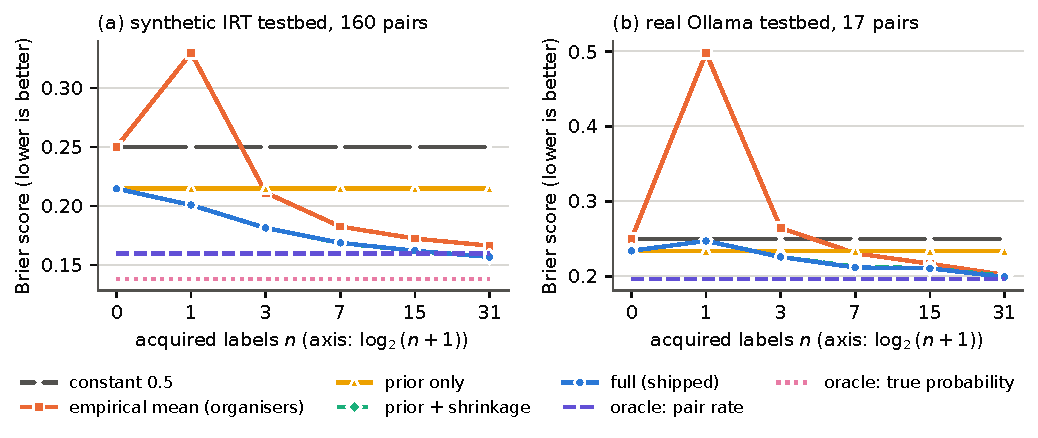
\includegraphics[width=\linewidth]{figures/brier_vs_budget}
\caption{Brier score per budget (the ALC of Eq.~\ref{eq:alc} is the trapezoidal area under these curves on the $\log_2(n{+}1)$ axis). The empirical mean is worse than the constant at $n=1$; shrinkage removes that penalty; the full model separates from shrinkage only at $n\ge15$. Dashed/dotted lines are the oracle references.}
\label{fig:budget}
\end{figure}

\paragraph{Main comparison.}
Table~\ref{tab:main} and Figure~\ref{fig:budget} give the headline numbers. On the real testbed the shipped predictor reaches \RFullAlc{} [\RFullAlcLo, \RFullAlcHi] against \REmpAlc{} [\REmpAlcLo, \REmpAlcHi] for the empirical mean and 0.25 for the constant; the paired difference to the empirical mean is \RPairFullEmpMean{} [\RPairFullEmpLo, \RPairFullEmpHi] (\RPairFullEmpSig; the full model is better on \RPairFullEmpFrac{} of pairs) and to the constant \RPairFullConstMean{} [\RPairFullConstLo, \RPairFullConstHi] (\RPairFullConstSig). On the synthetic testbed the corresponding ALCs are \SFullAlc{} [\SFullAlcLo, \SFullAlcHi] versus \SEmpAlc{} and 0.25, with paired differences \SPairFullEmpMean{} [\SPairFullEmpLo, \SPairFullEmpHi] and \SPairFullConstMean{} [\SPairFullConstLo, \SPairFullConstHi] (both \SPairFullConstSig). The empirical mean is \emph{worse} than the constant at $n=1$ on both testbeds ($B_1=\SEmpBOne$ and \REmpBOne) and only overtakes it from $n=\SEmpOvertake$ (synthetic) and $n=\REmpOvertake$ (real); on the real testbed its ALC (\REmpAlc) is \emph{above} the constant's 0.25 (paired difference \RPairEmpConstMean{} [\RPairEmpConstLo, \RPairEmpConstHi], \RPairEmpConstSig).

\paragraph{Where the gain comes from.}
Decomposing the ablation rows of Table~\ref{tab:main}: the prior alone improves on the constant by \SPairPriorConstMean{} (synthetic) and \RPairPriorConstMean{} (real) ALC; shrinkage adds \SPairShrinkPriorMean{} [\SPairShrinkPriorLo, \SPairShrinkPriorHi] and \RPairShrinkPriorMean{} [\RPairShrinkPriorLo, \RPairShrinkPriorHi] on top (the real-testbed difference is \RPairShrinkPriorSig{} with \RNPairs{} pairs). The item-level components are a much smaller effect. Against shrinkage, always-on $k$NN changes the ALC by \SPairKnnShrinkMean{} (synthetic) and \RPairKnnShrinkMean{} (real), always-on ridge by \SPairRidgeShrinkMean{} and \RPairRidgeShrinkMean, and the LOO-gated full model by \SPairFullShrinkMean{} [\SPairFullShrinkLo, \SPairFullShrinkHi] (\SPairFullShrinkSig) and \RPairFullShrinkMean{} [\RPairFullShrinkLo, \RPairFullShrinkHi] (\RPairFullShrinkSig); at $n=31$ alone the gated model changes the Brier score by \SPairFullShrinkBThirtyOneMean{} and \RPairFullShrinkBThirtyOneMean. Replacing TF-IDF by \texttt{\REmbModel} embeddings changes the full model's ALC by \REmbPairFullMean{} [\REmbPairFullLo, \REmbPairFullHi] (\REmbPairFullSig), so we ship TF-IDF; Appendix~\ref{app:ablations} adds the LOO gate against always-on components and a sharper unigram TF-IDF, which makes the $k$NN worse. We report these as what they are: item-level adaptation from at most 31 labels is a marginal gain whose sign has to be protected by the gate.

\paragraph{Headroom.}
The oracle rows explain why. On the synthetic testbed, knowing the true probability of every item gives an ALC of \SOrPAlc, knowing only the evaluation-set success rate \SOrRateAlc: perfect item-level discrimination is worth \SHeadroomItem{} ALC, to be recovered from 15--31 labels at budgets that carry 30\% of the weight. Shrinkage (\SShrinkAlc) is \SHeadroomRate{} above the rate oracle; that gap is the price of estimating a rate from few labels, concentrated at $n\le 3$ ($B_1$: \SHeadroomRateBOne; $B_{31}$: \SHeadroomRateBThirtyOne), and only a better prior, i.e.\ training data, can reduce it. On the real testbed the gap is \RHeadroomRate{} (\RShrinkAlc{} vs.\ \ROrRateAlc). The two parts of the headroom are of similar size but call for different remedies: a prior fitted to real subjects and benchmarks, and item difficulty information from outside the pair.

\paragraph{Prior strength and text signal.}
Figure~\ref{fig:sens} gives the ALC for $\alpha_0\in\{1,2,4,8\}$ (shrinkage is best at \SAlphaBestShrink{} on synthetic and \RAlphaBestShrink{} on real; full-model range \SAlphaFullRange{} and \RAlphaFullRange; we ship $\alpha_0=\CAlpha$, the smallest worst-case regret and the best of $\{2,4,8\}$ on the training release) and the synthetic sweep over $\sigma_{\mathrm{topic}}$, where the item-level effect stays two orders of magnitude below the item-level headroom (\SSweepAHeadroomItem{} to \SSweepEHeadroomItem): the gate protects against harm, it cannot create information.

\begin{figure}[t]
\centering
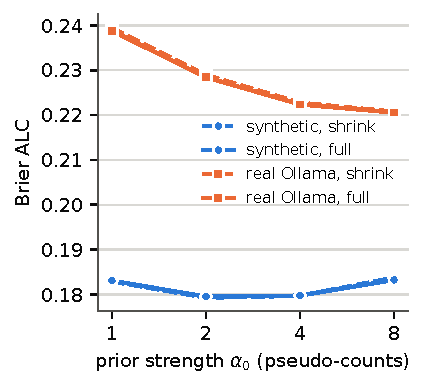
\includegraphics[width=0.38\linewidth]{figures/alpha0_sensitivity}\hfill
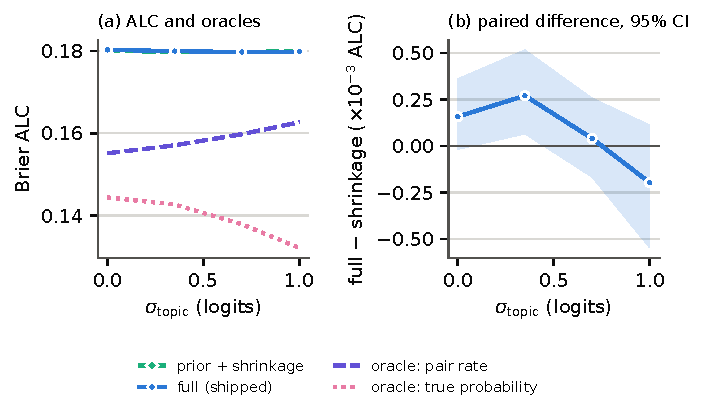
\includegraphics[width=0.59\linewidth]{figures/signal_sweep}
\caption{Left: Brier ALC vs.\ prior strength $\alpha_0$ (dashed: shrinkage, solid: full model). Right: synthetic sweep of the topic-difficulty spread $\sigma_{\mathrm{topic}}$ at $\gamma=0.3$: (a) ALC of shrinkage, the full model and the two oracles; (b) paired difference full $-$ shrinkage with its 95\% CI over pairs (negative favours the full model).}
\label{fig:sens}
\end{figure}

\paragraph{Acquisition policies.}
None of the five policies we compared is significantly different from the evaluator's random policy on either testbed (Appendix~\ref{app:ablations}, Table~\ref{tab:policies}): the shipped novelty filter gives \SPolNoveltyVsRandomMean{} [\SPolNoveltyVsRandomLo, \SPolNoveltyVsRandomHi] (synthetic) and \RPolNoveltyVsRandomMean{} [\RPolNoveltyVsRandomLo, \RPolNoveltyVsRandomHi] (real), the organisers' uncertainty band \SPolBleVsRandomMean{} and \RPolBleVsRandomMean. Selecting by $|p-0.5|$ distorts the pair-rate estimate that carries most of the metric; we ship the policy closest to random that removes near-duplicates.

\paragraph{Frontier-like subjects.}
The official test set has subjects our testbeds lack (2025--2026 releases, long reasoning efforts, very large models, agent harnesses); over \SensNGrid{} such descriptions the budget-0 prior ranges from \SensPMin{} to \SensPMax{} (the cap; Appendix~\ref{app:frontier}). What a wrong prior costs is exact under shrinkage (Table~\ref{tab:miscal}): a prior of $0.7$ on a pair whose true rate is $0.3$ costs \MiscalRThreePSeven{} ALC and loses to the constant (excess \MiscalConstRThreeExcess), whereas shrinkage beats the constant whenever $|r-0.5|\ge0.2$ and $|p_0-r|\le0.3$. On the real testbed an optimistic shift of every subject's prior logit costs significantly ($+0.5$: \ROffPlusHalfFullVsZeroMean), a pessimistic one does not ($-0.5$: \ROffMinusHalfFullVsZeroMean, \ROffMinusHalfFullVsZeroSig); on the training release the hand-set prior averages \FitHandPMean{} against a mean pair rate of \FitRateMean, so the intercept stays at zero.

\paragraph{Replication and calibration.}
Appendix~\ref{app:replication} reports replication over generator seeds and acquisition trajectories (the full model beats the empirical mean significantly in \RSeedsNFullEmpSig{} of \RSeedsN{} further real trajectories). Pooled ECE (Table~\ref{tab:main}) is \SFullEce/\RFullEce{} (synthetic/real) for the full model against \SEmpEce/\REmpEce{} for the empirical mean and \SConstEce/\RConstEce{} for the constant: shrinkage towards a sensible prior also fixes calibration at small budgets.

\section{Limitations}
\label{sec:limitations}

\emph{Local-versus-official gap.} Our real testbed covers four small open models on three benchmarks with two harnesses; the official test set contains frontier systems on many held-out benchmarks. In particular the subject part of the prior (release date, reasoning effort, size) has essentially no variance on our testbed and is validated only on the synthetic generator, whose attribute--ability relation we chose ourselves. Absolute ALC values will differ; we expect the \emph{ordering} shrinkage $>$ empirical mean $>$ constant at small budgets to transfer because it follows from the metric, but the sign and size of the item-level effects are testbed-dependent. \emph{A fitted prior did not help.} On the training release a logistic prior over the same visible attributes lost to the hand-set one under benchmark-held-out cross-validation, and an intercept-only prior lost by more: across benchmarks the pair success rate is dominated by benchmark difficulty, which the interface hides for test benchmarks, so visible subject attributes buy little at budget 0 and the gain over the empirical mean comes from shrinkage. Richer priors need information about the test benchmark itself. The most obvious source, the item text, did not provide it in our pre-registered test (hashed $n$-grams and text statistics, Section~\ref{sec:data}); pretrained text encoders remain untested, and labels of other subjects on the same benchmark are outside the stateless interface. \emph{Small real testbed.} \RNPairs{} pairs give wide confidence intervals; non-significant differences are stated as such. \emph{Stateless by design.} Labels are never pooled across subjects of the same benchmark (possible via \texttt{benchmark\_id}, but outside the spirit of the task). \emph{Weak text signal.} With at most 31 labels, lexical similarity recovers little of the item-level headroom on either testbed. \emph{Acquisition filter without measurable effect.} The novelty filter fires on templated real-testbed items (Appendix~\ref{app:ablations}) but changes the ALC by less than $10^{-4}$ relative to stream order; its value on heavily templated benchmarks is untested.

\section{Reproducibility}
\label{sec:repro}

All code, results and this report are released at \codeurl{} (also attached to the OpenReview submission). \texttt{experiments/src/model.py} and \texttt{labeling.py} are the shipped files; \texttt{build\_submission.py} creates the ZIP and runs the organisers' validator; \texttt{smoke\_test.py} checks interface and timing; \texttt{real\_testbed\_generate.py} regenerates the Ollama testbed; \texttt{simulate.py} is the IRT generator and \texttt{harness.py} the protocol; \texttt{run\_experiments.py --suite all}, \texttt{run\_extras.py}, \texttt{prior\_sensitivity.py}, \texttt{novelty\_stats.py}, \texttt{fit\_prior\_from\_measurement\_db.py} and \texttt{text\_prior.py} (round 3; its pre-registration and addendum are in \texttt{experiments/results/round3/}) write every result JSON in \texttt{experiments/results/}; \texttt{build\_paper.sh} runs \texttt{make\_macros.py}, \texttt{make\_figures.py} and \texttt{make\_audit.py} (which re-derives every directional claim of this report from the JSON files) and compiles the PDF, so no number is typed by hand. All seeds are fixed. Hardware: one laptop CPU (8 cores, 34 GB RAM, no GPU).

\section{Disclosure}
\label{sec:disclosure}

\emph{Training data:} the predictor has no fitted parameters. \texttt{aims-foundations/measurement-db} (revision \texttt{\FitRevisionShort}; the \texttt{subjects}, \texttt{items} and \texttt{responses} tables of its \FitNEligible{} competition-eligible benchmark directories, \FitNBench{} of which yielded usable pairs) was downloaded on 2026-10-22 with the author's account and used only (i) to evaluate the already-fixed shipped rule, (ii) to fit a candidate attribute prior and (iii) to train and cross-validate a candidate item-text prior on the \texttt{content} and \texttt{item\_features} of \TpNItems{} items, neither of which was shipped (Section~\ref{sec:data}; the \TpNBench{} benchmarks are listed in Appendix~\ref{app:textprior}); its traces and assets were not downloaded. No other source from the inventory was used. \emph{Evaluation data:} GSM8K and SVAMP test sets and ten BIG-Bench-Hard subtasks (local copies of the public Hugging Face datasets), used only to generate correctness labels of local models. \emph{Pretrained models:} Qwen2.5-Instruct 1.5B/3B/7B and Llama-3.2-3B-Instruct via Ollama, as evaluation subjects only; \texttt{sentence-transformers/all-MiniLM-L6-v2} in one offline ablation, not shipped. No commercial API was called. \emph{Compute:} a CPU-only laptop (8 cores, 34 GB RAM); about three hours of testbed generation, one hour for the experiment suite, one hour for the release fit, under an hour for the item-text prior. \emph{LLM coding assistant:} code, experiments and text were drafted by Anthropic's Claude (Claude Code) running autonomously on the author's machine; the author reviewed the pipeline and is responsible for the content.

\bibliographystyle{plainnat}
\bibliography{references}

\appendix

\section{Additional ablations}
\label{app:ablations}

\paragraph{Prior strength.}
Table~\ref{tab:alpha} gives the ALC for $\alpha_0\in\{1,2,4,8\}$. The best value differs between testbeds (shrinkage: \SAlphaBestShrink{} on synthetic, \RAlphaBestShrink{} on real), reflecting the wider spread of pair rates in the synthetic generator; the ALC of the full model varies by \SAlphaFullRange{} (synthetic) and \RAlphaFullRange{} (real) over the range, so the choice matters at the third decimal. On the training release $\alpha_0=4$ gives \FitRelHandAlphaFourAlc{} against \FitRelHandAlphaTwoAlc{} (2) and \FitRelHandAlphaEightAlc{} (8).

\paragraph{When does text help?}
The synthetic sweep (Figure~\ref{fig:sens}, right; Table~\ref{tab:sweep}) varies how much difficulty is explained by topic. With no topic or length signal ($\sigma_{\mathrm{topic}}=\SSweepASigma$, $\gamma=\SSweepAGamma$) the full model's paired difference to shrinkage is \SSweepAPairFullShrinkMean{} [\SSweepAPairFullShrinkLo, \SSweepAPairFullShrinkHi], the gate's cost when there is nothing to find; at the strongest setting ($\sigma_{\mathrm{topic}}=\SSweepESigma$) it is \SSweepEPairFullShrinkMean{} [\SSweepEPairFullShrinkLo, \SSweepEPairFullShrinkHi], while the item-level headroom (rate oracle minus true-probability oracle) grows from \SSweepAHeadroomItem{} to \SSweepEHeadroomItem.

\paragraph{Gating.}
Replacing the LOO gate by always-on components at their default settings gives \SLooAlwaysFullAlc{} versus \SLooGatedFullAlc{} (synthetic; paired gated$-$always \SLooPairGatedAlwaysMean{} [\SLooPairGatedAlwaysLo, \SLooPairGatedAlwaysHi], \SLooPairGatedAlwaysSig) and \RLooAlwaysFullAlc{} versus \RLooGatedFullAlc{} (real; \RLooPairGatedAlwaysMean{} [\RLooPairGatedAlwaysLo, \RLooPairGatedAlwaysHi], \RLooPairGatedAlwaysSig). The gate pays where always-on components overfit (the synthetic ridge) and costs a little where a component carries real signal (on the real testbed longer GSM8K problems are failed more often, which the always-on ridge exploits at $n\ge 15$); the second effect is within noise. Requiring 0, 1 or 2 standard errors of LOO improvement gives full-model ALCs of \SLooMultZeroFullAlc, \SLooMultOneFullAlc{} and \SLooMultTwoFullAlc{} (synthetic) and \RLooMultZeroFullAlc, \RLooMultOneFullAlc{} and \RLooMultTwoFullAlc{} (real); we ship the most conservative setting.

\paragraph{Sentence embeddings.}
The embeddings were computed offline for the real testbed (the model is on the validator's allow-list via \texttt{models.txt}, so it could have been shipped). They change the full model's ALC from \REmbTfidfFullAlc{} to \REmbMinilmFullAlc{} (paired \REmbPairFullMean{} [\REmbPairFullLo, \REmbPairFullHi], \REmbPairFullSig) and the always-on $k$NN variant from \REmbTfidfKnnAlc{} to \REmbMinilmKnnAlc{} (\REmbPairKnnMean{} [\REmbPairKnnLo, \REmbPairKnnHi], \REmbPairKnnSig), at the cost of a neural dependency, model loading and about 10~ms per embedding on CPU.

\paragraph{Sharper lexical similarity does not help.}
A unigram-only TF-IDF whose target terms are restricted to the acquired vocabulary separates same-topic from other-topic synthetic items far better (mean cosine about 0.3 versus 0.1 in the generator) but makes the always-on $k$NN \emph{worse}: paired against the shipped representation, the always-on $k$NN changes by \STfidfUniKnnVsShippedMean{} [\STfidfUniKnnVsShippedLo, \STfidfUniKnnVsShippedHi] (synthetic) and \RTfidfUniKnnVsShippedMean{} [\RTfidfUniKnnVsShippedLo, \RTfidfUniKnnVsShippedHi] (real), and the gated full model by \STfidfUniFullVsShippedMean{} [\STfidfUniFullVsShippedLo, \STfidfUniFullVsShippedHi] and \RTfidfUniFullVsShippedMean{} [\RTfidfUniFullVsShippedLo, \RTfidfUniFullVsShippedHi]. With a handful of neighbours per topic the kernel-weighted residual is dominated by label noise; the bigram-diluted similarity acts as a regulariser. Item-level signal exists (the oracles show it) but 31 labels are too few to exploit it through similarity alone.

\paragraph{Acquisition policies.}
Table~\ref{tab:policies} compares policies for the full predictor on identical pools and streams. Plain stream order differs from the evaluator's random policy by \SPolFirstVsRandomMean{} [\SPolFirstVsRandomLo, \SPolFirstVsRandomHi] (synthetic, \SPolFirstVsRandomSig) and \RPolFirstVsRandomMean{} [\RPolFirstVsRandomLo, \RPolFirstVsRandomHi] (real, \RPolFirstVsRandomSig)---both are uniform samples, so this is the trajectory-to-trajectory noise floor of the comparison. The shipped novelty filter gives \SPolNoveltyVsRandomMean{} [\SPolNoveltyVsRandomLo, \SPolNoveltyVsRandomHi] and \RPolNoveltyVsRandomMean{} [\RPolNoveltyVsRandomLo, \RPolNoveltyVsRandomHi]. It does fire on the real testbed: on \RNovPairsFired{} of \RNovNPairs{} pairs (\RNovSkipped{} candidates skipped in total, at most \RNovMaxSkipped{} per pair; templated BIG-Bench-Hard items such as \emph{navigate} and \emph{boolean expressions}, and SVAMP word problems sharing a template, reach cosine \RNovMaxSim), and on none of the \SNovNPairs{} synthetic pairs, whose pseudo-word items never get that similar---yet its ALC equals that of plain stream order to four decimals (\RPolNoveltyFullAlc{} vs.\ \RPolFirstFullAlc): skipping a near-duplicate changes which uniformly random items are labelled, not their distribution. The organisers' uncertainty band gives \SPolBleVsRandomMean{} [\SPolBleVsRandomLo, \SPolBleVsRandomHi] and \RPolBleVsRandomMean{} [\RPolBleVsRandomLo, \RPolBleVsRandomHi], and the novelty-plus-uncertainty variant \SPolNoveltyUncVsRandomMean{} and \RPolNoveltyUncVsRandomMean: selecting by $|p-0.5|$ reorders a near-random sample at small budgets and, once item-level corrections exist, biases it towards items of intermediate predicted difficulty, distorting the pair-rate estimate that carries most of the metric. None of the policies is significantly different from random on either testbed; we ship the one that is closest to random while removing redundant items.

\section{Replication}
\label{app:replication}
Regenerating the synthetic testbed with two further seeds gives full-model ALCs of \SSeedOneFullAlc{} and \SSeedTwoFullAlc{} (empirical mean \SSeedOneEmpAlc{} and \SSeedTwoEmpAlc; shrinkage \SSeedOneShrinkAlc{} and \SSeedTwoShrinkAlc). On the real testbed, four further acquisition trajectories give full-model ALCs between \RSeedsFullAlcMin{} and \RSeedsFullAlcMax{} (empirical mean \RSeedsEmpAlcMin--\RSeedsEmpAlcMax), and the full model beats the empirical mean significantly in \RSeedsNFullEmpSig{} of \RSeedsN{} trajectories. A $3\times3$ grid over the $k$NN scale and anchor ($\kappa\in\{1,2,4\}$, $\tau\in\{1,2,4\}$) spans \SGridBestFullAlc--\SGridWorstFullAlc{} on a smaller synthetic generator, i.e.\ the kernel constants matter little.

\section{Fitting pipeline details}
\label{app:fit}

\texttt{fit\_prior\_from\_measurement\_db.py} runs in five steps, each a sub-command. \emph{plan}: list the repository, download the small \texttt{benchmarks} table of every directory and keep those with \texttt{response\_type = binary} and \texttt{granularity = item} (the organisers' eligibility rule in \texttt{tools/prepare\_data.py}); record the bytes still to download and stop above a cap (30 GB by default). \emph{download}: fetch the eligible \texttt{subjects}, \texttt{items} and \texttt{responses} tables into the organisers' payload layout. \emph{fit}: build one row per (subject, test condition, item) with the mean response over trials as label (fractional labels enter as two weighted rows), each pair receiving total weight one; compute the subject and item terms with the shipped \texttt{model.subject\_terms} and \texttt{model.item\_terms}, so that fitted coefficients map one-to-one onto the constants of Section~\ref{sec:method}; add a one-hot for providers with at least 15 pairs and one for each training benchmark; fit an $L_2$-penalised logistic regression. Five-fold cross-validation holds out whole benchmarks; the penalty $C$ and the logit cap are selected by the pair-weighted budget-0 Brier score of the prior on held-out pairs, and $\alpha_0\in\{2,4,8\}$ by the closed-form shrinkage ALC of the protocol (50/50 split, 31 random acquisitions, Eq.~\ref{eq:alc}) on held-out pairs with at least 80 items, paired against the hand-set prior on the same pairs. \emph{testbeds}: evaluate the fitted table inside the harness on both local testbeds against the shipped constants. \emph{dry-run}: generate tables with the release schema (shared pool of subjects, random subsets per benchmark, benchmark difficulty offsets with standard deviation one logit, labels from a known coefficient table over the prior's own terms, two ineligible benchmarks) and run \emph{fit} on them. The dry run used \DryNBench{} eligible benchmarks, \DryNPairs{} pairs and \DryNRows{} rows; a light-regularisation fit recovers all \DryNSlopes{} slope signs with maximum error \DryMaxAbsErr{} and mean error \DryMeanAbsErr{} logits, and the fitted benchmark effects have standard deviation \DryBenchSd. Its cross-validated selection chose $C=\DrySelC$ and $\alpha_0=\DrySelAlpha$ and did not beat the hand-set prior (budget-0 Brier \DryPairBZeroMean{} [\DryPairBZeroLo, \DryPairBZeroHi]; shrinkage ALC \DryPairAlcMean{} [\DryPairAlcLo, \DryPairAlcHi]), so on these tables the rule would have kept the hand-set constants.

\paragraph{The run on the release.} Revision \texttt{\FitRevisionShort}; \FitNEligible{} eligible directories, \FitNBench{} with at least one pair of 20 or more distinct items; the pair unit is (benchmark directory, subject, test condition), since the release records several test conditions per subject on many benchmarks; \FitNPairs{} pairs, \FitNRows{} rows (each pair capped at \FitMaxItemsPerPair{} items); \FitNProviders{} providers with at least 15 pairs received a coefficient. Pair success rates have mean \FitRateMean{} and standard deviation \FitRateSd{} across pairs (benchmark means: standard deviation \FitBenchRateSd), while the hand-set $p_0$ has mean \FitHandPMean{} and standard deviation \FitHandPSd. The penalty grid ran from $C=\FitCMin$ to \FitCMax; the selection took $C=\FitSelC$, cap \FitSelCap{} and $\alpha_0=\FitSelAlpha$ (cross-validated budget-0 Brier \FitSelBZero, shrinkage ALC \FitSelAlc). The fitted benchmark effects have standard deviation \FitBenchEffectSd{} logits. Fitted vs.\ effective hand-set coefficients: release year \FitCoefYear{} vs.\ \HandEffCoefYear{} per year, size \FitCoefSize{} vs.\ \HandEffCoefSize{} per doubling, hard-tier cue \FitCoefTierHard{} vs.\ \HandEffCoefTierHard, easy-tier cue \FitCoefTierEasy{} vs.\ \HandEffCoefTierEasy, item length \FitCoefLength{} vs.\ \HandEffCoefLength; the reasoning-effort and harness terms shrink to about zero (\FitCoefEffortHigh, \FitCoefHarness; \FitFracPairsNoProvider{} of pairs carry no provider field and most carry no effort or harness field), and the provider table spans \FitProvMin{} (\texttt{\FitProvMinName}) to \FitProvMax{} (\texttt{\FitProvMaxName}). Inside the harness on the local testbeds the fitted table changes the full model's ALC by \FitRealPairFullMean{} [\FitRealPairFullLo, \FitRealPairFullHi] (real) and \FitSynPairFullMean{} [\FitSynPairFullLo, \FitSynPairFullHi] (synthetic); the result files are \texttt{prior\_fit.json} and \texttt{prior\_fit\_testbeds.json}, and the ship rule's verdict is recorded there (\FitShip).

\section{Item-text difficulty prior: details}
\label{app:textprior}

\paragraph{Pre-registration and outcome.} \texttt{experiments/results/round3/PREREG.md} (SHA-256 prefix \texttt{\TpPreregSha}, recorded in every result file and \TpPreregConsistent{} at build time) fixed features, target, model, nested selection, evaluation and ship rule before any text model was fitted. \texttt{PREREG\_ADDENDUM\_1.md} (\TpAddendumConsistent) registered the two exploratory variants after the primary folds had run, explicitly without influence on the decision. The rule: ship iff (a) the benchmark-held-out ALC difference (text minus hand-set) has a 95\% cluster-bootstrap CI below zero, (b) the real testbed is not significantly worse, and the engineering gates hold ($\ge200$ calls/s on one core with a new target item per call, weights $\le5$~MB, validator and smoke test pass, never raises). Outcome: (a) \TpRuleA, (b) \TpRuleB, gates \TpGates; the text prior is \TpShip.

\paragraph{Features and target.} JSON contents (the release stores many items as JSON objects) are flattened into \texttt{key: value} lines; words and word bigrams come from the first 2,000 characters (digit runs mapped to a length token), character trigrams from the first 500, and \texttt{item\_features} tokens form a fourth family; each family is sublinear-tf weighted and $\ell_2$-normalised, then hashed with \texttt{zlib.crc32} (sign from bit 31) into \TpBits{} buckets. The target of item $i$ is $\mathrm{logit}\,\frac{n_ir_i+0.5}{n_i+1}$ minus the mean hand-set subject logit of the $n_i$ pairs that evaluated it and minus its hand-set item logit, clipped to $\pm5$. At most 1,000 items per benchmark (\TpNTargetItems{} in total) are used for fitting; all \TpNItems{} items of the frame are scored (\TpNnz{} non-zeros). Exact duplicates of a test item's content in a training benchmark are rare (\TpDupMean\% of frame items on average), so shared items do not inflate the cross-validation.

\paragraph{Nested selection and fits.} In each outer fold a four-fold benchmark-grouped inner CV chooses the ridge penalty from $\{0.03,0.1,0.3,1,3,\TpAlphaGridMax\}$ by weighted MSE of the target; the inner out-of-fold scores give $W,B$ (pair-weighted logistic likelihood), the cap ($\{1.5,2.5,3.5\}$, training budget-0 Brier) and the within-pair weight $\lambda$ of the text offset ($\{0,0.5,1\}$, training closed-form ALC). Selected: penalty \TpFoldAlphas{} in every fold (the grid maximum), caps \TpFoldCaps, $\lambda=\TpFoldLambdas$, $W$ from \TpFoldWMin{} to \TpFoldWMax{} and $B$ from \TpFoldBMin{} to \TpFoldBMax. The held-out $R^2$ of the residual target was \TpFoldRsqMin{} to \TpFoldRsqMax{} across folds (inner CV: \TpInnerRsqMin{} to \TpInnerRsqMax). The final fit on all \TpNBench{} benchmarks again selected penalty \TpFinalAlpha{} with $W=\TpFinalW$, $B=\TpFinalB$, cap \TpFinalCap{} and $\lambda=\TpFinalLambda$; it is kept as \texttt{text\_prior\_candidate.json} (\TpFinalMB{} MB) and not shipped.

\begin{table}[htbp]
\caption{Item-text prior: benchmark-held-out cross-validation on the training release (closed-form protocol, shrinkage with $\alpha_0=4$ unless stated, no item-level components). $B_0$ over all items of each of the \TpNPairsBZero{} pairs; $B_1$--$B_7$ and ALC on the evaluation half of the \TpNPairsAlc{} pairs with at least 80 items. Exploratory rows were registered after the primary result; the oracles are references.}
\label{tab:textprior}
\centering\footnotesize
\begin{tabular}{lccccc}
\toprule
Method & $B_0$ & $B_1$ & $B_3$ & $B_7$ & ALC \\
\midrule
\rawinput results_table_textprior.tex
\bottomrule
\end{tabular}
\end{table}

\paragraph{Results.} Table~\ref{tab:textprior}. Per budget the paired differences are \TpDiffBudOneMean{} [\TpDiffBudOneLo, \TpDiffBudOneHi] at $n=1$ and \TpDiffBudThreeMean{} [\TpDiffBudThreeLo, \TpDiffBudThreeHi] at $n=3$ (gap to the pair-rate oracle closed: \TpGapOne\% [\TpGapOneLo, \TpGapOneHi] and \TpGapThree\% [\TpGapThreeLo, \TpGapThreeHi]); budget-0 Brier changes by \TpDiffBZeroMean{} [\TpDiffBZeroLo, \TpDiffBZeroHi]; the plain pair bootstrap gives \TpDiffAlcPairBootMean{} [\TpDiffAlcPairBootLo, \TpDiffAlcPairBootHi]. The text prior has the lower mean ALC in \TpFoldsBetter{} of \TpNFolds{} folds (significantly in \TpFoldsSigBetter) and on \TpBenchBetter{} of \TpBenchN{} benchmarks. Refitting only the intercept shift ($W=0$; a descriptive decomposition) gives \TpDiffIntShiftMean{} [\TpDiffIntShiftLo, \TpDiffIntShiftHi]: the hand-set prior's level is already right on held-out benchmarks. With the text prior, $\alpha_0=2$ gives \TpDiffAlphaTwoMean{} and $\alpha_0=8$ \TpDiffAlphaEightMean{} (\TpDiffAlphaEightSig) relative to the hand-set prior at $\alpha_0=4$. The exploratory variants (E1: grid \TpEOneGrid, selected \TpEOneAlphas; E2: statistics only, grid \TpETwoGrid, selected \TpETwoAlphas) changed the ALC by \TpEOneDiffMean{} [\TpEOneDiffLo, \TpEOneDiffHi] and \TpETwoDiffMean{} [\TpETwoDiffLo, \TpETwoDiffHi] and again had negative $W$ in \TpEOneNegW{} and \TpETwoNegW{} of \TpNFolds{} folds. The held-out benchmark-mean oracle closes \TpBenchOracleGapZero\%, \TpBenchOracleGapOne\% and \TpBenchOracleGapThree\% of the gap at $n=0,1,3$.

\paragraph{Local testbeds.} Full harness, identical trajectories: real ALC \TpRFullHand{} (hand-set) vs.\ \TpRFullText{} (text), paired \TpRPairFullMean{} [\TpRPairFullLo, \TpRPairFullHi], text better on \TpRPairFullFrac{} of pairs; without the BIG-Bench-Hard pairs, whose items may overlap the \texttt{fewshot\_ttt\_bbh} training benchmark, \TpRNoBbhMean{} [\TpRNoBbhLo, \TpRNoBbhHi] (\TpRNoBbhN{} pairs). Synthetic: \TpSFullHand{} vs.\ \TpSFullText{} (\TpSPairFullMean{} [\TpSPairFullLo, \TpSPairFullHi]); its pseudo-word items carry no transferable text signal by construction.

\paragraph{Engineering gates and the shipped file.} With the candidate loaded, \texttt{predict} runs at \TpCpsShort, \TpCpsMid{} and \TpCpsLong{} calls/s on one core with a new 15-, 300- and 2,000-word target item per call at budget 31 (the per-item text score is cached), the weights load in \TpLoadMs{} ms, and the smoke test passes \TpSmokeCases{} cases, including malformed JSON contents and a corrupted weight specification (which falls back to the hand-set prior); standard-library and numpy scores agree to \TpCheckMaxDiff. Since the rule failed, the submission ZIP is \TpZipUnchanged{} (SHA-256 prefix \texttt{\TpZipShaShort}); the development \texttt{model.py} keeps the text-prior hooks, which are inactive without a weight file and reproduce the shipped file's predictions bit for bit on \TpEquivSame{} of \TpEquivN{} test cases.

\paragraph{Benchmarks of the training release used (\TpNBench).} {\footnotesize \TpBenchList.}

\section{Prior sensitivity for frontier-like subjects}
\label{app:frontier}

Table~\ref{tab:frontier} gives the budget-0 prior $p_0$ of the shipped constants for subject descriptions that the official test set is likely to contain and our testbeds do not. Table~\ref{tab:miscal} gives the exact expected cost of a miscalibrated prior under the shipped shrinkage rule, and Table~\ref{tab:offset} the measured effect of shifting every subject's prior logit on the two testbeds (\texttt{PRIOR\_INTERCEPT} in \texttt{model.py}; all other constants unchanged; identical trajectories; generated by \texttt{prior\_sensitivity.py}).

\paragraph{Discussion.}
The official test set has subjects our testbeds lack (2025--2026 releases, long reasoning efforts, very large models, agent harnesses). Appendix~\ref{app:frontier} tabulates the budget-0 prior over \SensNGrid{} such descriptions: $p_0$ ranges from \SensPMin{} to \SensPMax{} (the cap); the organisers' GPT-4o and 2026 medium-effort sample subjects receive \SensPSampleGptFourO{} and \SensPSmokeSubject, our testbed models \SensPTestbedQwenSmall--\SensPTestbedLlama. What a wrong prior costs is exact: with $\alpha_0=\MiscalAlpha$ and $n$ labels the expected Brier excess over the pair-rate oracle is $\mathbb E[(\rho_n-r)^2]$ with binomial successes (Table~\ref{tab:miscal}). A prior of $0.7$ on a pair whose true rate is $0.3$ costs \MiscalRThreePSeven{} ALC and loses to the constant (excess \MiscalConstRThreeExcess); shrinkage beats the constant whenever $|r-0.5|\ge0.2$ and $|p_0-r|\le0.3$, and never when $|r-0.5|<0.15$, where the constant is close to optimal. Shifting every subject's prior logit by $\pm0.5$ or $\pm1$ (Table~\ref{tab:offset}) is asymmetric on the real testbed: $+0.5$ and $+1$ cost \ROffPlusHalfFullVsZeroMean{} and \ROffPlusOneFullVsZeroMean{} ALC (both significant), whereas $-0.5$ changes it by \ROffMinusHalfFullVsZeroMean{} [\ROffMinusHalfFullVsZeroLo, \ROffMinusHalfFullVsZeroHi] (\ROffMinusHalfFullVsZeroSig)---small models at \RAccMin--\RAccMax\% accuracy tolerate a pessimistic prior; on the synthetic testbed zero is best and both $\pm0.5$ shifts cost significantly (\SOffMinusHalfFullVsZeroMean, \SOffPlusHalfFullVsZeroMean). On the training release the hand-set prior averages \FitHandPMean{} against a mean pair rate of \FitRateMean, i.e.\ it is not optimistic for real systems. We keep the intercept at zero and name it as the first constant to change if the official formative score points the other way.

\begin{table}[htbp]
\caption{Budget-0 prior $p_0$ (no item cues; 600-character item) by release year and \texttt{reasoning\_effort} for a subject with no size or name cue on the default harness (left), and for a high-effort subject on a non-default harness with a \emph{mini} name cue, a 70B or a 400B parameter count (right). The organisers' sample subjects receive \SensPSampleGptFourO{} (GPT-4o, 2024-05) and \SensPSmokeSubject{} (2026-01, medium effort, non-default harness).}
\label{tab:frontier}
\centering\small
\begin{tabular}{lcccc|ccc}
\toprule
& \multicolumn{4}{c}{default harness, no name cue} & \multicolumn{3}{c}{high effort, non-default harness} \\
Release year & none & low & medium & high & mini & 70B & 400B \\
\midrule
\rawinput results_table_frontier.tex
\bottomrule
\end{tabular}
\end{table}

\begin{table}[htbp]
\caption{Exact expected Brier ALC excess over the pair-rate oracle $r(1-r)$ of the shipped shrinkage rule ($\alpha_0=\MiscalAlpha$, clipping to $[\CClipLo,\CClipHi]$) when the prior rate is $p_0$ and the true pair rate is $r$; the number of successes among the $n$ acquired labels is binomial$(n,r)$ and the ALC weights are those of Eq.~\ref{eq:alc}. The last column is the excess of the constant 0.5; $^{\dagger}$ marks cells where the constant is better.}
\label{tab:miscal}
\centering\small\setlength{\tabcolsep}{5pt}
\begin{tabular}{l|cccccc|c}
\toprule
& \multicolumn{6}{c|}{prior rate $p_0$} & \\
True rate $r$ & 0.3 & 0.4 & 0.5 & 0.6 & 0.7 & 0.8 & constant 0.5 \\
\midrule
\rawinput results_table_miscal.tex
\bottomrule
\end{tabular}
\end{table}

\begin{table}[htbp]
\caption{Brier ALC of the prior alone, shrinkage and the full model when every subject's prior logit is shifted by \texttt{PRIOR\_INTERCEPT} (random policy, same trajectories as Table~\ref{tab:main}). The shipped value is 0.}
\label{tab:offset}
\centering\small
\begin{tabular}{l|ccc|ccc}
\toprule
& \multicolumn{3}{c|}{Real Ollama (\RNPairs{} pairs)} & \multicolumn{3}{c}{Synthetic IRT (\SNPairs{} pairs)} \\
Shift (logits) & prior & shrinkage & full & prior & shrinkage & full \\
\midrule
\rawinput results_table_offset.tex
\bottomrule
\end{tabular}
\end{table}

\section{Validator and smoke-test output}
The organisers' validator exits with code 0 and prints
\begin{center}\texttt{OK: paiec\_submission.zip looks like a valid submission ZIP.}\end{center}
(full output in \texttt{experiments/results/validator\_output.txt}; ZIP SHA-256 prefix \texttt{\ZipShaShort}). The smoke test (\texttt{experiments/results/smoke\_test.json}) records \SmokeNCases{} successful cases and the timings quoted in Section~\ref{sec:impl}.

\section{Additional tables}

\begin{table}[htbp]
\caption{Acquisition policies (full predictor): Brier ALC [95\% CI] and paired difference to the evaluator's random policy on the same pairs (negative favours the policy). The BLE rule accepts a candidate when its current prediction satisfies $|p-0.5|\le0.15$~\citep{paiec_baselines_2026}.}
\label{tab:policies}
\centering\footnotesize\setlength{\tabcolsep}{3pt}
\resizebox{\linewidth}{!}{%
\begin{tabular}{lllll}
\toprule
& \multicolumn{2}{c}{Synthetic} & \multicolumn{2}{c}{Real} \\
Policy & ALC [95\% CI] & $\Delta$ vs random [95\% CI] & ALC [95\% CI] & $\Delta$ vs random [95\% CI] \\
\midrule
\rawinput results_table_policies.tex
\bottomrule
\end{tabular}}
\end{table}

\begin{table}[htbp]
\caption{Real Ollama testbed: one pair per (model, harness, benchmark). Accuracy is the success rate over all items of the pair (acquisition and evaluation pools together).}
\label{tab:testbed}
\centering\small
\begin{tabular}{lllrr}
\toprule
Model (Ollama tag) & Harness & Benchmark & Items & Acc.\ (\%) \\
\midrule
\rawinput results_table_testbed.tex
\bottomrule
\end{tabular}
\end{table}

\begin{table}[htbp]
\caption{Brier score per budget for the main methods (random policy). The last column is the ALC of Eq.~\ref{eq:alc}.}
\label{tab:budget}
\centering\small
\begin{tabular}{llcccccc|c}
\toprule
Testbed & Method & $B_0$ & $B_1$ & $B_3$ & $B_7$ & $B_{15}$ & $B_{31}$ & ALC \\
\midrule
\rawinput results_table_budget.tex
\bottomrule
\end{tabular}
\end{table}

\begin{table}[htbp]
\caption{Synthetic signal sweep (\SNPairs{} pairs per setting, seed 0): ALC of shrinkage and of the full model, their paired difference, and the two oracle references.}
\label{tab:sweep}
\centering\footnotesize\setlength{\tabcolsep}{4pt}
\begin{tabular}{cclllll}
\toprule
$\sigma_{\mathrm{topic}}$ & $\gamma$ & Shrinkage & Full [95\% CI] & Full $-$ shrink [95\% CI] & Oracle rate & Oracle $p$ \\
\midrule
\rawinput results_table_sweep.tex
\bottomrule
\end{tabular}
\end{table}

\begin{table}[htbp]
\caption{Sensitivity to the prior strength $\alpha_0$ (Brier ALC).}
\label{tab:alpha}
\centering\small
\begin{tabular}{lcccc}
\toprule
& $\alpha_0=1$ & $\alpha_0=2$ & $\alpha_0=4$ & $\alpha_0=8$ \\
\midrule
Synthetic, shrinkage & \SAlphaOneShrinkAlc & \SAlphaTwoShrinkAlc & \SAlphaFourShrinkAlc & \SAlphaEightShrinkAlc \\
Synthetic, full & \SAlphaOneFullAlc & \SAlphaTwoFullAlc & \SAlphaFourFullAlc & \SAlphaEightFullAlc \\
Real, shrinkage & \RAlphaOneShrinkAlc & \RAlphaTwoShrinkAlc & \RAlphaFourShrinkAlc & \RAlphaEightShrinkAlc \\
Real, full & \RAlphaOneFullAlc & \RAlphaTwoFullAlc & \RAlphaFourFullAlc & \RAlphaEightFullAlc \\
\bottomrule
\end{tabular}
\end{table}

\end{document}
